%&preformat-disser
\RequirePackage[l2tabu,orthodox]{nag} % Раскомментировав, можно в логе получать рекомендации относительно правильного использования пакетов и предупреждения об устаревших и нерекомендуемых пакетах
% Формат А4, 14pt (ГОСТ Р 7.0.11-2011, 5.3.6)
\documentclass[a4paper,14pt,oneside,openany]{memoir}

%%%%%%%%%%%%%%%%%%%%%%%%%%%%%%%%%%%%%%%%%%%%%%%%%%%%%%
%%%% Файл упрощённых настроек шаблона диссертации %%%%
%%%%%%%%%%%%%%%%%%%%%%%%%%%%%%%%%%%%%%%%%%%%%%%%%%%%%%

%%% Инициализирование переменных, не трогать!  %%%
\newcounter{intvl}
\newcounter{otstup}
\newcounter{contnumeq}
\newcounter{contnumfig}
\newcounter{contnumtab}
\newcounter{pgnum}
\newcounter{chapstyle}
\newcounter{headingdelim}
\newcounter{headingalign}
\newcounter{headingsize}
\newcounter{tabcap}
\newcounter{tablaba}
\newcounter{tabtita}
\newcounter{usefootcite}
%%%%%%%%%%%%%%%%%%%%%%%%%%%%%%%%%%%%%%%%%%%%%%%%%%

%%% Область упрощённого управления оформлением %%%

%% Интервал между заголовками и между заголовком и текстом
% Заголовки отделяют от текста сверху и снизу тремя интервалами (ГОСТ Р 7.0.11-2011, 5.3.5)
\setcounter{intvl}{3}               % Коэффициент кратности к размеру шрифта

%% Отступы у заголовков в тексте
\setcounter{otstup}{0}              % 0 --- без отступа; 1 --- абзацный отступ

%% Нумерация формул, таблиц и рисунков
\setcounter{contnumeq}{0}           % Нумерация формул: 0 --- пораздельно (во введении подряд, без номера раздела); 1 --- сквозная нумерация по всей диссертации
\setcounter{contnumfig}{0}          % Нумерация рисунков: 0 --- пораздельно (во введении подряд, без номера раздела); 1 --- сквозная нумерация по всей диссертации
\setcounter{contnumtab}{1}          % Нумерация таблиц: 0 --- пораздельно (во введении подряд, без номера раздела); 1 --- сквозная нумерация по всей диссертации

%% Оглавление
\setcounter{pgnum}{1}               % 0 --- номера страниц никак не обозначены; 1 --- Стр. над номерами страниц (дважды компилировать после изменения)
\settocdepth{subsection}            % до какого уровня подразделов выносить в оглавление
\setsecnumdepth{subsection}         % до какого уровня нумеровать подразделы


%% Текст и форматирование заголовков
\setcounter{chapstyle}{1}           % 0 --- разделы только под номером; 1 --- разделы с названием "Глава" перед номером
\setcounter{headingdelim}{1}        % 0 --- номер отделен пропуском в 1em или \quad; 1 --- номера разделов и приложений отделены точкой с пробелом, подразделы пропуском без точки; 2 --- номера разделов, подразделов и приложений отделены точкой с пробелом.

%% Выравнивание заголовков в тексте
\setcounter{headingalign}{0}        % 0 --- по центру; 1 --- по левому краю

%% Размеры заголовков в тексте
\setcounter{headingsize}{0}         % 0 --- по ГОСТ, все всегда 14 пт; 1 --- пропорционально изменяющийся размер в зависимости от базового шрифта

%% Подпись таблиц
\setcounter{tabcap}{0}              % 0 --- по ГОСТ, номер таблицы и название разделены тире, выровнены по левому краю, при необходимости на нескольких строках; 1 --- подпись таблицы не по ГОСТ, на двух и более строках, дальнейшие настройки: 
%Выравнивание первой строки, с подписью и номером
\setcounter{tablaba}{2}             % 0 --- по левому краю; 1 --- по центру; 2 --- по правому краю
%Выравнивание строк с самим названием таблицы
\setcounter{tabtita}{1}             % 0 --- по левому краю; 1 --- по центру; 2 --- по правому краю
%Разделитель записи «Таблица #» и названия таблицы
\newcommand{\tablabelsep}{ }

%% Подпись рисунков
%Разделитель записи «Рисунок #» и названия рисунка
\newcommand{\figlabelsep}{~\cyrdash\ } % (ГОСТ 2.105, 4.3.1) % "--- здесь не работает

%%% Цвета гиперссылок %%%
% Latex color definitions: http://latexcolor.com/
%\definecolor{linkcolor}{rgb}{0.9,0,0}
%\definecolor{citecolor}{rgb}{0,0.6,0}
%\definecolor{urlcolor}{rgb}{0,0,1}
\definecolor{linkcolor}{rgb}{0,0,0} %black
\definecolor{citecolor}{rgb}{0,0,0} %black
\definecolor{urlcolor}{rgb}{0,0,0} %black
               % общие настройки шаблона
%%% Проверка используемого TeX-движка %%%
\RequirePackage{ifxetex, ifluatex}
\newif\ifxetexorluatex   % определяем новый условный оператор (http://tex.stackexchange.com/a/47579)
\ifxetex
    \xetexorluatextrue
\else
    \ifluatex
        \xetexorluatextrue
    \else
        \xetexorluatexfalse
    \fi
\fi

\newif\ifsynopsis           % Условие, проверяющее, что документ --- автореферат

\RequirePackage{etoolbox}[2015/08/02]               % Для продвинутой проверки разных условий

%%% Поля и разметка страницы %%%
\usepackage{pdflscape}                              % Для включения альбомных страниц
\usepackage{geometry}                               % Для последующего задания полей

%%% Математические пакеты %%%
\usepackage{amsthm,amsmath,amscd}       % Математические дополнения от AMS
\ifxetexorluatex
    \usepackage{amsfonts,amssymb}       % Математические дополнения от AMS
\else
    \ifnumequal{\value{usealtfont}}{2}{}{
        \usepackage{amsfonts,amssymb}       % Математические дополнения от AMS
    }
\fi
\usepackage{mathtools}                  % Добавляет окружение multlined

%%%% Установки для размера шрифта 14 pt %%%%
%% Формирование переменных и констант для сравнения (один раз для всех подключаемых файлов)%%
%% должно располагаться до вызова пакета fontspec или polyglossia, потому что они сбивают его работу
\newlength{\curtextsize}
\newlength{\bigtextsize}
\setlength{\bigtextsize}{14pt}

\makeatletter
%\show\f@size                                       % неплохо для отслеживания, но вызывает стопорение процесса, если документ компилируется без команды  -interaction=nonstopmode 
\setlength{\curtextsize}{\f@size pt}
\makeatother

%%% Кодировки и шрифты %%%
\ifxetexorluatex
    \usepackage{polyglossia}[2014/05/21]            % Поддержка многоязычности (fontspec подгружается автоматически)
\else
   %%% Решение проблемы копирования текста в буфер кракозябрами
    \ifnumequal{\value{usealtfont}}{1}{% Используется pscyr, при наличии
        \IfFileExists{pscyr.sty}{% вероятно, без pscyr нет необходимости в этом коде
            \input glyphtounicode.tex
            \input glyphtounicode-cmr.tex %from pdfx package
            \pdfgentounicode=1
        }{}
    }{}
    \usepackage{cmap}                               % Улучшенный поиск русских слов в полученном pdf-файле
    \defaulthyphenchar=127                          % Если стоит до fontenc, то переносы не впишутся в выделяемый текст при копировании его в буфер обмена 
    \usepackage[T1,T2A]{fontenc}                    % Поддержка русских букв
    \ifnumequal{\value{usealtfont}}{1}{% Используется pscyr, при наличии
        \IfFileExists{pscyr.sty}{\usepackage{pscyr}}{}  % Подключение pscyr
    }{}
    \usepackage[utf8]{inputenc}[2014/04/30]         % Кодировка utf8
    \usepackage[english, russian]{babel}[2014/03/24]% Языки: русский, английский
    \ifnumequal{\value{usealtfont}}{2}{
        % http://dxdy.ru/post1238763.html#p1238763
        \usepackage[scaled=0.925]{XCharter}[2017/06/25] % Подключение русифицированных шрифтов XCharter
        \usepackage[bitstream-charter]{mathdesign} % Согласование математических шрифтов
    }{}
\fi

%%% Оформление абзацев %%%
\usepackage{indentfirst}                            % Красная строка

%%% Цвета %%%
\usepackage[dvipsnames, table, hyperref, cmyk]{xcolor} % Совместимо с tikz. Конвертация всех цветов в cmyk заложена как удовлетворение возможного требования типографий. Возможно конвертирование и в rgb.

%%% Таблицы %%%
\usepackage{longtable,ltcaption}                    % Длинные таблицы
\usepackage{multirow,makecell}                      % Улучшенное форматирование таблиц

%%% Общее форматирование
\usepackage{soulutf8}                               % Поддержка переносоустойчивых подчёркиваний и зачёркиваний
\usepackage{icomma}                                 % Запятая в десятичных дробях
\usepackage[hyphenation, lastparline]{impnattypo}   % Оптимизация расстановки переносов и длины последней строки абзаца

%%% Гиперссылки %%%
\usepackage{hyperref}[2012/11/06]

%%% Изображения %%%
\usepackage{graphicx}[2014/04/25]                   % Подключаем пакет работы с графикой

%%% Списки %%%
\usepackage{enumitem}

%%% Счётчики %%%
\usepackage[figure,table]{totalcount}               % Счётчик рисунков и таблиц
\usepackage{totcount}                               % Пакет создания счётчиков на основе последнего номера подсчитываемого элемента (может требовать дважды компилировать документ)
\usepackage{totpages}                               % Счётчик страниц, совместимый с hyperref (ссылается на номер последней страницы). Желательно ставить последним пакетом в преамбуле

%%% Продвинутое управление групповыми ссылками (пока только формулами) %%%
\ifxetexorluatex
    \usepackage{cleveref}                           % cleveref корректно считывает язык из настроек polyglossia
\else
    \usepackage[russian]{cleveref}                  % cleveref имеет сложности со считыванием языка из babel. Такое решение русификации вывода выбрано вместо определения в documentclass из опасности что-то лишнее передать во все остальные пакеты, включая библиографию.
\fi
\creflabelformat{equation}{#2#1#3}                  % Формат по умолчанию ставил круглые скобки вокруг каждого номера ссылки, теперь просто номера ссылок без какого-либо дополнительного оформления
\crefrangelabelformat{equation}{#3#1#4\cyrdash#5#2#6}   % Интервалы в русском языке принято делать через тире, если иное не оговорено


\ifnumequal{\value{draft}}{1}{% Черновик
    \usepackage[firstpage]{draftwatermark}
    \SetWatermarkText{DRAFT}
    \SetWatermarkFontSize{14pt}
    \SetWatermarkScale{15}
    \SetWatermarkAngle{45}
}{}

%%% Цитата, не приводимая в автореферате:
% возможно, актуальна только для biblatex
%\newcommand{\citeinsynopsis}[1]{\ifsynopsis\else ~\cite{#1} \fi}
  % Пакеты общие для диссертации и автореферата
\synopsisfalse                           % Этот документ --- не автореферат
%%% Прикладные пакеты %%% 
%\usepackage{calc}               % Пакет для расчётов параметров, например длины

%%% Для добавления Стр. над номерами страниц в оглавлении
%%% http://tex.stackexchange.com/a/306950
\usepackage{afterpage}

%%% Для добавления псевдокода в текст диссертации
\usepackage{algorithm}
\usepackage{algpseudocode}

\usepackage{svg}

\usepackage{tikz}                   % Продвинутый пакет векторной графики
\usetikzlibrary{chains}             % Для примера tikz рисунка
\usetikzlibrary{shapes.geometric}   % Для примера tikz рисунка
\usetikzlibrary{shapes.symbols}     % Для примера tikz рисунка
\usetikzlibrary{arrows}             % Для примера tikz рисунка
\ifnumequal{\value{imgprecompile}}{1}{% Только если у нас включена предкомпиляция
    \usetikzlibrary{external}   % подключение возможности предкомпиляции
    \tikzexternalize[prefix=Dissertation/images/] % activate! % здесь можно указать отдельную папку для скомпилированных файлов
}{}
         % Пакеты для диссертации
\input{Dissertation/userpackages}        % Пакеты для специфических пользовательских задач

%%%%%%%%%%%%%%%%%%%%%%%%%%%%%%%%%%%%%%%%%%%%%%%%%%%%%%
%%%% Файл упрощённых настроек шаблона диссертации %%%%
%%%%%%%%%%%%%%%%%%%%%%%%%%%%%%%%%%%%%%%%%%%%%%%%%%%%%%

%%% Инициализирование переменных, не трогать!  %%%
\newcounter{intvl}
\newcounter{otstup}
\newcounter{contnumeq}
\newcounter{contnumfig}
\newcounter{contnumtab}
\newcounter{pgnum}
\newcounter{chapstyle}
\newcounter{headingdelim}
\newcounter{headingalign}
\newcounter{headingsize}
\newcounter{tabcap}
\newcounter{tablaba}
\newcounter{tabtita}
\newcounter{usefootcite}
%%%%%%%%%%%%%%%%%%%%%%%%%%%%%%%%%%%%%%%%%%%%%%%%%%

%%% Область упрощённого управления оформлением %%%

%% Интервал между заголовками и между заголовком и текстом
% Заголовки отделяют от текста сверху и снизу тремя интервалами (ГОСТ Р 7.0.11-2011, 5.3.5)
\setcounter{intvl}{3}               % Коэффициент кратности к размеру шрифта

%% Отступы у заголовков в тексте
\setcounter{otstup}{0}              % 0 --- без отступа; 1 --- абзацный отступ

%% Нумерация формул, таблиц и рисунков
\setcounter{contnumeq}{0}           % Нумерация формул: 0 --- пораздельно (во введении подряд, без номера раздела); 1 --- сквозная нумерация по всей диссертации
\setcounter{contnumfig}{0}          % Нумерация рисунков: 0 --- пораздельно (во введении подряд, без номера раздела); 1 --- сквозная нумерация по всей диссертации
\setcounter{contnumtab}{1}          % Нумерация таблиц: 0 --- пораздельно (во введении подряд, без номера раздела); 1 --- сквозная нумерация по всей диссертации

%% Оглавление
\setcounter{pgnum}{1}               % 0 --- номера страниц никак не обозначены; 1 --- Стр. над номерами страниц (дважды компилировать после изменения)
\settocdepth{subsection}            % до какого уровня подразделов выносить в оглавление
\setsecnumdepth{subsection}         % до какого уровня нумеровать подразделы


%% Текст и форматирование заголовков
\setcounter{chapstyle}{1}           % 0 --- разделы только под номером; 1 --- разделы с названием "Глава" перед номером
\setcounter{headingdelim}{1}        % 0 --- номер отделен пропуском в 1em или \quad; 1 --- номера разделов и приложений отделены точкой с пробелом, подразделы пропуском без точки; 2 --- номера разделов, подразделов и приложений отделены точкой с пробелом.

%% Выравнивание заголовков в тексте
\setcounter{headingalign}{0}        % 0 --- по центру; 1 --- по левому краю

%% Размеры заголовков в тексте
\setcounter{headingsize}{0}         % 0 --- по ГОСТ, все всегда 14 пт; 1 --- пропорционально изменяющийся размер в зависимости от базового шрифта

%% Подпись таблиц
\setcounter{tabcap}{0}              % 0 --- по ГОСТ, номер таблицы и название разделены тире, выровнены по левому краю, при необходимости на нескольких строках; 1 --- подпись таблицы не по ГОСТ, на двух и более строках, дальнейшие настройки: 
%Выравнивание первой строки, с подписью и номером
\setcounter{tablaba}{2}             % 0 --- по левому краю; 1 --- по центру; 2 --- по правому краю
%Выравнивание строк с самим названием таблицы
\setcounter{tabtita}{1}             % 0 --- по левому краю; 1 --- по центру; 2 --- по правому краю
%Разделитель записи «Таблица #» и названия таблицы
\newcommand{\tablabelsep}{ }

%% Подпись рисунков
%Разделитель записи «Рисунок #» и названия рисунка
\newcommand{\figlabelsep}{~\cyrdash\ } % (ГОСТ 2.105, 4.3.1) % "--- здесь не работает

%%% Цвета гиперссылок %%%
% Latex color definitions: http://latexcolor.com/
%\definecolor{linkcolor}{rgb}{0.9,0,0}
%\definecolor{citecolor}{rgb}{0,0.6,0}
%\definecolor{urlcolor}{rgb}{0,0,1}
\definecolor{linkcolor}{rgb}{0,0,0} %black
\definecolor{citecolor}{rgb}{0,0,0} %black
\definecolor{urlcolor}{rgb}{0,0,0} %black
               % Упрощённые настройки шаблона

\input{Dissertation/preamblenames}       % Переопределение именований, чтобы можно было и в преамбуле использовать
% Новые переменные, которые могут использоваться во всём проекте
% ГОСТ 7.0.11-2011
% 9.2 Оформление текста автореферата диссертации
% 9.2.1 Общая характеристика работы включает в себя следующие основные структурные
% элементы:
% актуальность темы исследования;
\newcommand{\actualityTXT}{Актуальность темы.}
% степень ее разработанности;
\newcommand{\progressTXT}{Степень разработанности темы.}
% объект и предмет исследования
\newcommand{\objectTXT}{Объектом исследования}
\newcommand{\subjectTXT}{Предметом исследования}
% цели и задачи;
\newcommand{\aimTXT}{Целью}
\newcommand{\tasksTXT}{задачи}
% научную новизну;
\newcommand{\noveltyTXT}{Научная новизна:}
% теоретическую и практическую значимость работы;
%\newcommand{\influenceTXT}{Теоретическая и практическая значимость}
% или чаще используют просто
\newcommand{\influenceTXT}{Практическая значимость}
% методологию и методы исследования;
\newcommand{\methodsTXT}{Mетодология и методы исследования.}
% положения, выносимые на защиту;
\newcommand{\defpositionsTXT}{Основные положения, выносимые на~защиту:}
% степень достоверности и апробацию результатов.
\newcommand{\reliabilityTXT}{Достоверность}
\newcommand{\probationTXT}{Апробация работы.}

\newcommand{\contributionTXT}{Личный вклад.}
\newcommand{\publicationsTXT}{Публикации.}


\newcommand{\authorbibtitle}{Публикации автора по теме диссертации}
\newcommand{\vakbibtitle}{В изданиях из списка ВАК РФ}
\newcommand{\notvakbibtitle}{В прочих изданиях}
\newcommand{\confbibtitle}{В сборниках трудов конференций}
\newcommand{\fullbibtitle}{Список литературы} % (ГОСТ Р 7.0.11-2011, 4)
  % Новые переменные, которые могут использоваться во всём проекте

%%% Основные сведения %%%
\newcommand{\thesisAuthorLastName}{Матрохин}
\newcommand{\thesisAuthorOtherNames}{Дмитрий Александрович}
\newcommand{\thesisAuthorInitials}{Д.\,А.}
\newcommand{\thesisAuthor}             % Диссертация, ФИО автора
{%
    \texorpdfstring{% \texorpdfstring takes two arguments and uses the first for (La)TeX and the second for pdf
        \thesisAuthorLastName~\thesisAuthorOtherNames% так будет отображаться на титульном листе или в тексте, где будет использоваться переменная
    }{%
        \thesisAuthorLastName, \thesisAuthorOtherNames% эта запись для свойств pdf-файла. В таком виде, если pdf будет обработан программами для сбора библиографических сведений, будет правильно представлена фамилия.
    }
}
\newcommand{\thesisAuthorShort}        % Диссертация, ФИО автора инициалами
{\thesisAuthorInitials~\thesisAuthorLastName}
\newcommand{\thesisAuthorGroup}{ИПОВС-21}

%\newcommand{\thesisUdk}                % Диссертация, УДК
%{\todo{xxx.xxx}}
\newcommand{\thesisTitle}              % Диссертация, название
{Исследование и разработка алгоритма построения выпуклой оболочки для вычисления дескрипторов объектов на изображении}
\newcommand{\thesisSpecialtyNumber}    % Диссертация, специальность, номер
{09.04.04}
\newcommand{\thesisSpecialtyTitle}     % Диссертация, специальность, название
{Программная инженерия}
\newcommand{\thesisSpecialtyProgram}{Программное обеспечение автоматизированных систем и вычислительных комплексов}

\newcommand{\thesisCity}               % Диссертация, город написания диссертации
{Москва}
\newcommand{\thesisYear}               % Диссертация, год написания диссертации
{2018}
\newcommand{\thesisOrganization}       % Диссертация, организация
{Федеральное государственное автономное образовательное учреждение высшего образования «Национальный исследовательский университет «Московский институт электронной техники»}
\newcommand{\thesisOrganizationShort}  % Диссертация, краткое название организации для доклада
{\todo{НИУ «МИЭТ»}}

\newcommand{\faculty}{микроприборов и технической кибернетики}
\newcommand{\department}{информатики и программного обеспечения вычислительных систем}

\newcommand{\thesisInOrganization}     % Диссертация, организация в предложном падеже: Работа выполнена в ...
{\todo{учреждении, в~котором выполнялась данная диссертационная работа}}

\newcommand{\supervisorFio}            % Научный руководитель, ФИО
{Дорогов Виктор Георгиевич}
\newcommand{\supervisorRegalia}        % Научный руководитель, регалии
{к.т.н.\,~доцент}
\newcommand{\supervisorFioShort}       % Научный руководитель, ФИО
{В.\,Г.~Дорогов}
\newcommand{\supervisorRegaliaShort}   % Научный руководитель, регалии
{\todo{к.т.н.\,~доцент}}


\newcommand{\opponentOneFio}           % Оппонент 1, ФИО
{\todo{Фамилия Имя Отчество}}
\newcommand{\opponentOneRegalia}       % Оппонент 1, регалии
{\todo{доктор физико-математических наук, профессор}}
\newcommand{\opponentOneJobPlace}      % Оппонент 1, место работы
{\todo{Не очень длинное название для места работы}}
\newcommand{\opponentOneJobPost}       % Оппонент 1, должность
{\todo{старший научный сотрудник}}

\newcommand{\opponentTwoFio}           % Оппонент 2, ФИО
{\todo{Фамилия Имя Отчество}}
\newcommand{\opponentTwoRegalia}       % Оппонент 2, регалии
{\todo{кандидат физико-математических наук}}
\newcommand{\opponentTwoJobPlace}      % Оппонент 2, место работы
{\todo{Основное место работы c длинным длинным длинным длинным названием}}
\newcommand{\opponentTwoJobPost}       % Оппонент 2, должность
{\todo{старший научный сотрудник}}

\newcommand{\leadingOrganizationTitle} % Ведущая организация, дополнительные строки
{\todo{Федеральное государственное бюджетное образовательное учреждение высшего профессионального образования с~длинным длинным длинным длинным названием}}

\newcommand{\defenseDate}              % Защита, дата
{\todo{DD mmmmmmmm YYYY~г.~в~XX часов}}
\newcommand{\defenseCouncilNumber}     % Защита, номер диссертационного совета
{\todo{Д\,123.456.78}}
\newcommand{\defenseCouncilTitle}      % Защита, учреждение диссертационного совета
{\todo{Название учреждения}}
\newcommand{\defenseCouncilAddress}    % Защита, адрес учреждение диссертационного совета
{\todo{Адрес}}
\newcommand{\defenseCouncilPhone}      % Телефон для справок
{\todo{+7~(0000)~00-00-00}}

\newcommand{\defenseSecretaryFio}      % Секретарь диссертационного совета, ФИО
{\todo{Фамилия Имя Отчество}}
\newcommand{\defenseSecretaryRegalia}  % Секретарь диссертационного совета, регалии
{\todo{д-р~физ.-мат. наук}}            % Для сокращений есть ГОСТы, например: ГОСТ Р 7.0.12-2011 + http://base.garant.ru/179724/#block_30000

\newcommand{\synopsisLibrary}          % Автореферат, название библиотеки
{\todo{Название библиотеки}}
\newcommand{\synopsisDate}             % Автореферат, дата рассылки
{\todo{DD mmmmmmmm YYYY года}}

% To avoid conflict with beamer class use \providecommand
\providecommand{\keywords}%            % Ключевые слова для метаданных PDF диссертации и автореферата
{}
      % Основные сведения
\input{common/styles}    % Стили общие для диссертации и автореферата
%%% Изображения %%%
\graphicspath{{images/}{Dissertation/images/}}         % Пути к изображениям

%%% Макет страницы %%%
% Выставляем значения полей (ГОСТ 7.0.11-2011, 5.3.7)
\geometry{a4paper,top=2cm,bottom=1.5cm,left=3cm,right=1.5cm,nofoot,nomarginpar} %,showframe
\setlength{\topskip}{0pt}   %размер дополнительного верхнего поля
\setlength{\footskip}{0pt} % снимет warning, согласно https://tex.stackexchange.com/a/334346

%%% Интервалы %%%
%% По ГОСТ Р 7.0.11-2011, пункту 5.3.6 требуется полуторный интервал
%% Реализация средствами класса (на основе setspace) ближе к типографской классике.
%% И правит сразу и в таблицах (если со звёздочкой) 
%\DoubleSpacing*     % Двойной интервал
\OnehalfSpacing*    % Полуторный интервал
\setSpacing{1.42}   % Полуторный интервал, подобный Ворду (возможно, стоит включать вместе с предыдущей строкой)

%%% Выравнивание и переносы %%%
%% http://tex.stackexchange.com/questions/241343/what-is-the-meaning-of-fussy-sloppy-emergencystretch-tolerance-hbadness
%% http://www.latex-community.org/forum/viewtopic.php?p=70342#p70342
\tolerance 1414
\hbadness 1414
\emergencystretch 1.5em % В случае проблем регулировать в первую очередь
\hfuzz 0.3pt
\vfuzz \hfuzz
%\raggedbottom
%\sloppy                 % Избавляемся от переполнений
\clubpenalty=10000      % Запрещаем разрыв страницы после первой строки абзаца
\widowpenalty=10000     % Запрещаем разрыв страницы после последней строки абзаца

%%% Блок управления параметрами для выравнивания заголовков в тексте %%%
\newlength{\otstuplen}
\setlength{\otstuplen}{\theotstup\parindent}
\ifnumequal{\value{headingalign}}{0}{% выравнивание заголовков в тексте
    \newcommand{\hdngalign}{\centering}                % по центру
    \newcommand{\hdngaligni}{}% по центру
    \setlength{\otstuplen}{0pt}
}{%
    \newcommand{\hdngalign}{}                 % по левому краю
    \newcommand{\hdngaligni}{\hspace{\otstuplen}}      % по левому краю
} % В обоих случаях вроде бы без переноса, как и надо (ГОСТ Р 7.0.11-2011, 5.3.5)

%%% Оглавление %%%
\renewcommand{\cftchapterdotsep}{\cftdotsep}                % отбивка точками до номера страницы начала главы/раздела

%% Переносить слова в заголовке не допускается (ГОСТ Р 7.0.11-2011, 5.3.5). Заголовки в оглавлении должны точно повторять заголовки в тексте (ГОСТ Р 7.0.11-2011, 5.2.3). Прямого указания на запрет переносов в оглавлении нет, но по той же логике невнесения искажений в смысл, лучше в оглавлении не переносить:
\setrmarg{2.55em plus1fil}                             %To have the (sectional) titles in the ToC, etc., typeset ragged right with no hyphenation
\renewcommand{\cftchapterpagefont}{\normalfont}        % нежирные номера страниц у глав в оглавлении
\renewcommand{\cftchapterleader}{\cftdotfill{\cftchapterdotsep}}% нежирные точки до номеров страниц у глав в оглавлении
%\renewcommand{\cftchapterfont}{}                       % нежирные названия глав в оглавлении

\ifnumgreater{\value{headingdelim}}{0}{%
    \renewcommand\cftchapteraftersnum{.\space}       % добавляет точку с пробелом после номера раздела в оглавлении
}{}
\ifnumgreater{\value{headingdelim}}{1}{%
    \renewcommand\cftsectionaftersnum{.\space}       % добавляет точку с пробелом после номера подраздела в оглавлении
    \renewcommand\cftsubsectionaftersnum{.\space}    % добавляет точку с пробелом после номера подподраздела в оглавлении
    \renewcommand\cftsubsubsectionaftersnum{.\space} % добавляет точку с пробелом после номера подподподраздела в оглавлении
    \AtBeginDocument{% без этого polyglossia сама всё переопределяет
        \setsecnumformat{\csname the#1\endcsname.\space}
    }
}{%
    \AtBeginDocument{% без этого polyglossia сама всё переопределяет
        \setsecnumformat{\csname the#1\endcsname\quad}
    }
}

\renewcommand*{\cftappendixname}{\appendixname\space} % Слово Приложение в оглавлении

%%% Колонтитулы %%%
% Порядковый номер страницы печатают на середине верхнего поля страницы (ГОСТ Р 7.0.11-2011, 5.3.8)
\makeevenhead{plain}{}{}{}
\makeoddhead{plain}{}{}{}
\makeevenfoot{plain}{}{\thepage}{}
\makeoddfoot{plain}{}{\thepage}{}
\pagestyle{plain}

%%% добавить Стр. над номерами страниц в оглавлении
%%% http://tex.stackexchange.com/a/306950
\newif\ifendTOC

\newcommand*{\tocheader}{
\ifnumequal{\value{pgnum}}{1}{%
    \ifendTOC\else\hbox to \linewidth%
      {\noindent{}~\hfill{Стр.}}\par%
      \ifnumless{\value{page}}{3}{}{%
        \vspace{0.5\onelineskip}
      }
      \afterpage{\tocheader}
    \fi%
}{}%
}%

%%% Оформление заголовков глав, разделов, подразделов %%%
%% Работа должна быть выполнена ... размером шрифта 12-14 пунктов (ГОСТ Р 7.0.11-2011, 5.3.8). То есть не должно быть надписей шрифтом более 14. Так и поставим.
%% Эти установки будут давать одинаковый результат независимо от выбора базовым шрифтом 12 пт или 14 пт
\newcommand{\basegostsectionfont}{\fontsize{14pt}{16pt}\selectfont\bfseries}

\makechapterstyle{thesisgost}{%
    \chapterstyle{default}
    \setlength{\beforechapskip}{0pt}
    \setlength{\midchapskip}{0pt}
    \setlength{\afterchapskip}{\theintvl\curtextsize}
    \renewcommand*{\chapnamefont}{\basegostsectionfont}
    \renewcommand*{\chapnumfont}{\basegostsectionfont}
    \renewcommand*{\chaptitlefont}{\basegostsectionfont}
    \renewcommand*{\chapterheadstart}{}
    \ifnumgreater{\value{headingdelim}}{0}{%
        \renewcommand*{\afterchapternum}{.\space}   % добавляет точку с пробелом после номера раздела
    }{%
        \renewcommand*{\afterchapternum}{\quad}     % добавляет \quad после номера раздела
    }
    \renewcommand*{\printchapternum}{\hdngaligni\hdngalign\chapnumfont \thechapter}
    \renewcommand*{\printchaptername}{}
    \renewcommand*{\printchapternonum}{\hdngaligni\hdngalign}
}

\makeatletter
\makechapterstyle{thesisgostchapname}{%
    \chapterstyle{thesisgost}
    \renewcommand*{\printchapternum}{\chapnumfont \thechapter}
    \renewcommand*{\printchaptername}{\hdngaligni\hdngalign\chapnamefont \@chapapp} %
}
\makeatother

\chapterstyle{thesisgost}

\setsecheadstyle{\basegostsectionfont\hdngalign}
\setsecindent{\otstuplen}

\setsubsecheadstyle{\basegostsectionfont\hdngalign}
\setsubsecindent{\otstuplen}

\setsubsubsecheadstyle{\basegostsectionfont\hdngalign}
\setsubsubsecindent{\otstuplen}

\sethangfrom{\noindent #1} %все заголовки подразделов центрируются с учетом номера, как block 

\ifnumequal{\value{chapstyle}}{1}{%
    \chapterstyle{thesisgostchapname}
    \renewcommand*{\cftchaptername}{\chaptername\space} % будет вписано слово Глава перед каждым номером раздела в оглавлении
}{}%

%%% Интервалы между заголовками
\setbeforesecskip{\theintvl\curtextsize}% Заголовки отделяют от текста сверху и снизу тремя интервалами (ГОСТ Р 7.0.11-2011, 5.3.5).
\setaftersecskip{\theintvl\curtextsize}
\setbeforesubsecskip{\theintvl\curtextsize}
\setaftersubsecskip{\theintvl\curtextsize}
\setbeforesubsubsecskip{\theintvl\curtextsize}
\setaftersubsubsecskip{\theintvl\curtextsize}

%%% Блок дополнительного управления размерами заголовков
\ifnumequal{\value{headingsize}}{1}{% Пропорциональные заголовки и базовый шрифт 14 пт
    \renewcommand{\basegostsectionfont}{\large\bfseries}
    \renewcommand*{\chapnamefont}{\Large\bfseries}
    \renewcommand*{\chapnumfont}{\Large\bfseries}
    \renewcommand*{\chaptitlefont}{\Large\bfseries}
}{}

%%% Счётчики %%%

%% Упрощённые настройки шаблона диссертации: нумерация формул, таблиц, рисунков
\ifnumequal{\value{contnumeq}}{1}{%
    \counterwithout{equation}{chapter} % Убираем связанность номера формулы с номером главы/раздела
}{}
\ifnumequal{\value{contnumfig}}{1}{%
    \counterwithout{figure}{chapter}   % Убираем связанность номера рисунка с номером главы/раздела
}{}
\ifnumequal{\value{contnumtab}}{1}{%
    \counterwithout{table}{chapter}    % Убираем связанность номера таблицы с номером главы/раздела
}{}


%%http://www.linux.org.ru/forum/general/6993203#comment-6994589 (используется totcount)
\makeatletter
\def\formbytotal#1#2#3#4#5{%
    \newcount\@c
    \@c\totvalue{#1}\relax
    \newcount\@last
    \newcount\@pnul
    \@last\@c\relax
    \divide\@last 10
    \@pnul\@last\relax
    \divide\@pnul 10
    \multiply\@pnul-10
    \advance\@pnul\@last
    \multiply\@last-10
    \advance\@last\@c
    \total{#1}~#2%
    \ifnum\@pnul=1#5\else%
    \ifcase\@last#5\or#3\or#4\or#4\or#4\else#5\fi
    \fi
}
\makeatother

\AtBeginDocument{
%% регистрируем счётчики в системе totcounter
    \regtotcounter{totalcount@figure}
    \regtotcounter{totalcount@table}       % Если иным способом поставить в преамбуле то ошибка в числе таблиц
    \regtotcounter{TotPages}               % Если иным способом поставить в преамбуле то ошибка в числе страниц
}

%%% Правильная нумерация приложений %%%
%% По ГОСТ 2.105, п. 4.3.8 Приложения обозначают заглавными буквами русского алфавита,
%% начиная с А, за исключением букв Ё, З, Й, О, Ч, Ь, Ы, Ъ.
%% Здесь также переделаны все нумерации русскими буквами.
\ifxetexorluatex
    \makeatletter
    \def\russian@Alph#1{\ifcase#1\or
       А\or Б\or В\or Г\or Д\or Е\or Ж\or
       И\or К\or Л\or М\or Н\or
       П\or Р\or С\or Т\or У\or Ф\or Х\or
       Ц\or Ш\or Щ\or Э\or Ю\or Я\else\xpg@ill@value{#1}{russian@Alph}\fi}
    \def\russian@alph#1{\ifcase#1\or
       а\or б\or в\or г\or д\or е\or ж\or
       и\or к\or л\or м\or н\or
       п\or р\or с\or т\or у\or ф\or х\or
       ц\or ш\or щ\or э\or ю\or я\else\xpg@ill@value{#1}{russian@alph}\fi}
    \makeatother
\else
    \makeatletter
    \if@uni@ode
      \def\russian@Alph#1{\ifcase#1\or
        А\or Б\or В\or Г\or Д\or Е\or Ж\or
        И\or К\or Л\or М\or Н\or
        П\or Р\or С\or Т\or У\or Ф\or Х\or
        Ц\or Ш\or Щ\or Э\or Ю\or Я\else\@ctrerr\fi}
    \else
      \def\russian@Alph#1{\ifcase#1\or
        \CYRA\or\CYRB\or\CYRV\or\CYRG\or\CYRD\or\CYRE\or\CYRZH\or
        \CYRI\or\CYRK\or\CYRL\or\CYRM\or\CYRN\or
        \CYRP\or\CYRR\or\CYRS\or\CYRT\or\CYRU\or\CYRF\or\CYRH\or
        \CYRC\or\CYRSH\or\CYRSHCH\or\CYREREV\or\CYRYU\or
        \CYRYA\else\@ctrerr\fi}
    \fi
    \if@uni@ode
      \def\russian@alph#1{\ifcase#1\or
        а\or б\or в\or г\or д\or е\or ж\or
        и\or к\or л\or м\or н\or
        п\or р\or с\or т\or у\or ф\or х\or
        ц\or ш\or щ\or э\or ю\or я\else\@ctrerr\fi}
    \else
      \def\russian@alph#1{\ifcase#1\or
        \cyra\or\cyrb\or\cyrv\or\cyrg\or\cyrd\or\cyre\or\cyrzh\or
        \cyri\or\cyrk\or\cyrl\or\cyrm\or\cyrn\or
        \cyrp\or\cyrr\or\cyrs\or\cyrt\or\cyru\or\cyrf\or\cyrh\or
        \cyrc\or\cyrsh\or\cyrshch\or\cyrerev\or\cyryu\or
        \cyrya\else\@ctrerr\fi}
    \fi
    \makeatother
\fi           % Стили для диссертации
% для вертикального центрирования ячеек в tabulary
\def\zz{\ifx\[$\else\aftergroup\zzz\fi}
%$ \] % <-- чиним подсветку синтаксиса в некоторых редакторах
\def\zzz{\setbox0\lastbox
\dimen0\dimexpr\extrarowheight + \ht0-\dp0\relax
\setbox0\hbox{\raise-.5\dimen0\box0}%
\ht0=\dimexpr\ht0+\extrarowheight\relax
\dp0=\dimexpr\dp0+\extrarowheight\relax 
\box0
}



\lstdefinelanguage{Renhanced}%
{keywords={abbreviate,abline,abs,acos,acosh,action,add1,add,%
        aggregate,alias,Alias,alist,all,anova,any,aov,aperm,append,apply,%
        approx,approxfun,apropos,Arg,args,array,arrows,as,asin,asinh,%
        atan,atan2,atanh,attach,attr,attributes,autoload,autoloader,ave,%
        axis,backsolve,barplot,basename,besselI,besselJ,besselK,besselY,%
        beta,binomial,body,box,boxplot,break,browser,bug,builtins,bxp,by,%
        c,C,call,Call,case,cat,category,cbind,ceiling,character,char,%
        charmatch,check,chol,chol2inv,choose,chull,class,close,cm,codes,%
        coef,coefficients,co,col,colnames,colors,colours,commandArgs,%
        comment,complete,complex,conflicts,Conj,contents,contour,%
        contrasts,contr,control,helmert,contrib,convolve,cooks,coords,%
        distance,coplot,cor,cos,cosh,count,fields,cov,covratio,wt,CRAN,%
        create,crossprod,cummax,cummin,cumprod,cumsum,curve,cut,cycle,D,%
        data,dataentry,date,dbeta,dbinom,dcauchy,dchisq,de,debug,%
        debugger,Defunct,default,delay,delete,deltat,demo,de,density,%
        deparse,dependencies,Deprecated,deriv,description,detach,%
        dev2bitmap,dev,cur,deviance,off,prev,,dexp,df,dfbetas,dffits,%
        dgamma,dgeom,dget,dhyper,diag,diff,digamma,dim,dimnames,dir,%
        dirname,dlnorm,dlogis,dnbinom,dnchisq,dnorm,do,dotplot,double,%
        download,dpois,dput,drop,drop1,dsignrank,dt,dummy,dump,dunif,%
        duplicated,dweibull,dwilcox,dyn,edit,eff,effects,eigen,else,%
        emacs,end,environment,env,erase,eval,equal,evalq,example,exists,%
        exit,exp,expand,expression,External,extract,extractAIC,factor,%
        fail,family,fft,file,filled,find,fitted,fivenum,fix,floor,for,%
        For,formals,format,formatC,formula,Fortran,forwardsolve,frame,%
        frequency,ftable,ftable2table,function,gamma,Gamma,gammaCody,%
        gaussian,gc,gcinfo,gctorture,get,getenv,geterrmessage,getOption,%
        getwd,gl,glm,globalenv,gnome,GNOME,graphics,gray,grep,grey,grid,%
        gsub,hasTsp,hat,heat,help,hist,home,hsv,httpclient,I,identify,if,%
        ifelse,Im,image,\%in\%,index,influence,measures,inherits,install,%
        installed,integer,interaction,interactive,Internal,intersect,%
        inverse,invisible,IQR,is,jitter,kappa,kronecker,labels,lapply,%
        layout,lbeta,lchoose,lcm,legend,length,levels,lgamma,library,%
        licence,license,lines,list,lm,load,local,locator,log,log10,log1p,%
        log2,logical,loglin,lower,lowess,ls,lsfit,lsf,ls,machine,Machine,%
        mad,mahalanobis,make,link,margin,match,Math,matlines,mat,matplot,%
        matpoints,matrix,max,mean,median,memory,menu,merge,methods,min,%
        missing,Mod,mode,model,response,mosaicplot,mtext,mvfft,na,nan,%
        names,omit,nargs,nchar,ncol,NCOL,new,next,NextMethod,nextn,%
        nlevels,nlm,noquote,NotYetImplemented,NotYetUsed,nrow,NROW,null,%
        numeric,\%o\%,objects,offset,old,on,Ops,optim,optimise,optimize,%
        options,or,order,ordered,outer,package,packages,page,pairlist,%
        pairs,palette,panel,par,parent,parse,paste,path,pbeta,pbinom,%
        pcauchy,pchisq,pentagamma,persp,pexp,pf,pgamma,pgeom,phyper,pico,%
        pictex,piechart,Platform,plnorm,plogis,plot,pmatch,pmax,pmin,%
        pnbinom,pnchisq,pnorm,points,poisson,poly,polygon,polyroot,pos,%
        postscript,power,ppoints,ppois,predict,preplot,pretty,Primitive,%
        print,prmatrix,proc,prod,profile,proj,prompt,prop,provide,%
        psignrank,ps,pt,ptukey,punif,pweibull,pwilcox,q,qbeta,qbinom,%
        qcauchy,qchisq,qexp,qf,qgamma,qgeom,qhyper,qlnorm,qlogis,qnbinom,%
        qnchisq,qnorm,qpois,qqline,qqnorm,qqplot,qr,Q,qty,qy,qsignrank,%
        qt,qtukey,quantile,quasi,quit,qunif,quote,qweibull,qwilcox,%
        rainbow,range,rank,rbeta,rbind,rbinom,rcauchy,rchisq,Re,read,csv,%
        csv2,fwf,readline,socket,real,Recall,rect,reformulate,regexpr,%
        relevel,remove,rep,repeat,replace,replications,report,require,%
        resid,residuals,restart,return,rev,rexp,rf,rgamma,rgb,rgeom,R,%
        rhyper,rle,rlnorm,rlogis,rm,rnbinom,RNGkind,rnorm,round,row,%
        rownames,rowsum,rpois,rsignrank,rstandard,rstudent,rt,rug,runif,%
        rweibull,rwilcox,sample,sapply,save,scale,scan,scan,screen,sd,se,%
        search,searchpaths,segments,seq,sequence,setdiff,setequal,set,%
        setwd,show,sign,signif,sin,single,sinh,sink,solve,sort,source,%
        spline,splinefun,split,sqrt,stars,start,stat,stem,step,stop,%
        storage,strstrheight,stripplot,strsplit,structure,strwidth,sub,%
        subset,substitute,substr,substring,sum,summary,sunflowerplot,svd,%
        sweep,switch,symbol,symbols,symnum,sys,status,system,t,table,%
        tabulate,tan,tanh,tapply,tempfile,terms,terrain,tetragamma,text,%
        time,title,topo,trace,traceback,transform,tri,trigamma,trunc,try,%
        ts,tsp,typeof,unclass,undebug,undoc,union,unique,uniroot,unix,%
        unlink,unlist,unname,untrace,update,upper,url,UseMethod,var,%
        variable,vector,Version,vi,warning,warnings,weighted,weights,%
        which,while,window,write,\%x\%,x11,X11,xedit,xemacs,xinch,xor,%
        xpdrows,xy,xyinch,yinch,zapsmall,zip},%
    otherkeywords={!,!=,~,$,*,\%,\&,\%/\%,\%*\%,\%\%,<-,<<-},%$
    alsoother={._$},%$
    sensitive,%
    morecomment=[l]\#,%
    morestring=[d]",%
    morestring=[d]'% 2001 Robert Denham
}%

%решаем проблему с кириллицей в комментариях (в pdflatex) https://tex.stackexchange.com/a/103712/79756
\lstset{extendedchars=true,literate={Ö}{{\"O}}1
    {Ä}{{\"A}}1
    {Ü}{{\"U}}1
    {ß}{{\ss}}1
    {ü}{{\"u}}1
    {ä}{{\"a}}1
    {ö}{{\"o}}1
    {~}{{\textasciitilde}}1
    {а}{{\selectfont\char224}}1
    {б}{{\selectfont\char225}}1
    {в}{{\selectfont\char226}}1
    {г}{{\selectfont\char227}}1
    {д}{{\selectfont\char228}}1
    {е}{{\selectfont\char229}}1
    {ё}{{\"e}}1
    {ж}{{\selectfont\char230}}1
    {з}{{\selectfont\char231}}1
    {и}{{\selectfont\char232}}1
    {й}{{\selectfont\char233}}1
    {к}{{\selectfont\char234}}1
    {л}{{\selectfont\char235}}1
    {м}{{\selectfont\char236}}1
    {н}{{\selectfont\char237}}1
    {о}{{\selectfont\char238}}1
    {п}{{\selectfont\char239}}1
    {р}{{\selectfont\char240}}1
    {с}{{\selectfont\char241}}1
    {т}{{\selectfont\char242}}1
    {у}{{\selectfont\char243}}1
    {ф}{{\selectfont\char244}}1
    {х}{{\selectfont\char245}}1
    {ц}{{\selectfont\char246}}1
    {ч}{{\selectfont\char247}}1
    {ш}{{\selectfont\char248}}1
    {щ}{{\selectfont\char249}}1
    {ъ}{{\selectfont\char250}}1
    {ы}{{\selectfont\char251}}1
    {ь}{{\selectfont\char252}}1
    {э}{{\selectfont\char253}}1
    {ю}{{\selectfont\char254}}1
    {я}{{\selectfont\char255}}1
    {А}{{\selectfont\char192}}1
    {Б}{{\selectfont\char193}}1
    {В}{{\selectfont\char194}}1
    {Г}{{\selectfont\char195}}1
    {Д}{{\selectfont\char196}}1
    {Е}{{\selectfont\char197}}1
    {Ё}{{\"E}}1
    {Ж}{{\selectfont\char198}}1
    {З}{{\selectfont\char199}}1
    {И}{{\selectfont\char200}}1
    {Й}{{\selectfont\char201}}1
    {К}{{\selectfont\char202}}1
    {Л}{{\selectfont\char203}}1
    {М}{{\selectfont\char204}}1
    {Н}{{\selectfont\char205}}1
    {О}{{\selectfont\char206}}1
    {П}{{\selectfont\char207}}1
    {Р}{{\selectfont\char208}}1
    {С}{{\selectfont\char209}}1
    {Т}{{\selectfont\char210}}1
    {У}{{\selectfont\char211}}1
    {Ф}{{\selectfont\char212}}1
    {Х}{{\selectfont\char213}}1
    {Ц}{{\selectfont\char214}}1
    {Ч}{{\selectfont\char215}}1
    {Ш}{{\selectfont\char216}}1
    {Щ}{{\selectfont\char217}}1
    {Ъ}{{\selectfont\char218}}1
    {Ы}{{\selectfont\char219}}1
    {Ь}{{\selectfont\char220}}1
    {Э}{{\selectfont\char221}}1
    {Ю}{{\selectfont\char222}}1
    {Я}{{\selectfont\char223}}1
    {і}{{\selectfont\char105}}1
    {ї}{{\selectfont\char168}}1
    {є}{{\selectfont\char185}}1
    {ґ}{{\selectfont\char160}}1
    {І}{{\selectfont\char73}}1
    {Ї}{{\selectfont\char136}}1
    {Є}{{\selectfont\char153}}1
    {Ґ}{{\selectfont\char128}}1
}

% Ширина текста минус ширина надписи 999
\newlength{\twless}
\newlength{\lmarg}
\setlength{\lmarg}{\widthof{999}}   % ширина надписи 999
\setlength{\twless}{\textwidth-\lmarg}


\lstset{ %
%    language=R,                     %  Язык указать здесь, если во всех листингах преимущественно один язык, в результате часть настроек может пойти только для этого языка
    numbers=left,                   % where to put the line-numbers
    numberstyle=\fontsize{12pt}{14pt}\selectfont\color{Gray},  % the style that is used for the line-numbers
    firstnumber=1,                  % в этой и следующей строках задаётся поведение нумерации 5, 10, 15...
    stepnumber=5,                   % the step between two line-numbers. If it's 1, each line will be numbered
    numbersep=5pt,                  % how far the line-numbers are from the code
    backgroundcolor=\color{white},  % choose the background color. You must add \usepackage{color}
    showspaces=false,               % show spaces adding particular underscores
    showstringspaces=false,         % underline spaces within strings
    showtabs=false,                 % show tabs within strings adding particular underscores
    frame=leftline,                 % adds a frame of different types around the code
    rulecolor=\color{black},        % if not set, the frame-color may be changed on line-breaks within not-black text (e.g. commens (green here))
    tabsize=2,                      % sets default tabsize to 2 spaces
    captionpos=t,                   % sets the caption-position to top
    breaklines=true,                % sets automatic line breaking
    breakatwhitespace=false,        % sets if automatic breaks should only happen at whitespace
%    title=\lstname,                 % show the filename of files included with \lstinputlisting;
    % also try caption instead of title
    basicstyle=\fontsize{12pt}{14pt}\selectfont\ttfamily,% the size of the fonts that are used for the code
%    keywordstyle=\color{blue},      % keyword style
    commentstyle=\color{ForestGreen}\emph,% comment style
    stringstyle=\color{Mahogany},   % string literal style
    escapeinside={\%*}{*)},         % if you want to add a comment within your code
    morekeywords={*,...},           % if you want to add more keywords to the set
    inputencoding=utf8,             % кодировка кода
    xleftmargin={\lmarg},           % Чтобы весь код и полоска с номерами строк была смещена влево, так чтобы цифры не вылезали за пределы текста слева
} 

%http://tex.stackexchange.com/questions/26872/smaller-frame-with-listings
% Окружение, чтобы листинг был компактнее обведен рамкой, если она задается, а не на всю ширину текста
\makeatletter
\newenvironment{SmallListing}[1][]
{\lstset{#1}\VerbatimEnvironment\begin{VerbatimOut}{VerbEnv.tmp}}
{\end{VerbatimOut}\settowidth\@tempdima{%
        \lstinputlisting{VerbEnv.tmp}}
    \minipage{\@tempdima}\lstinputlisting{VerbEnv.tmp}\endminipage}    
\makeatother


\DefineVerbatimEnvironment% с шрифтом 12 пт
{Verb}{Verbatim}
{fontsize=\fontsize{12pt}{14pt}\selectfont}

%\newfloat[chapter]{ListingEnv}{lol}{Листинг}

\renewcommand{\lstlistingname}{Листинг}

%Общие счётчики окружений листингов
%http://tex.stackexchange.com/questions/145546/how-to-make-figure-and-listing-share-their-counter
% Если смешивать плавающие и не плавающие окружения, то могут быть проблемы с нумерацией
\makeatletter
\AtBeginDocument{%
    \let\c@ListingEnv\c@lstlisting
    \let\theListingEnv\thelstlisting
    \let\ftype@lstlisting\ftype@ListingEnv % give the floats the same precedence
}
\makeatother

% значок С++ — используйте команду \cpp
\newcommand{\cpp}{%
    C\nolinebreak\hspace{-.05em}%
    \raisebox{.2ex}{+}\nolinebreak\hspace{-.10em}%
    \raisebox{.2ex}{+}%
}

%%%  Чересстрочное форматирование таблиц
%% http://tex.stackexchange.com/questions/278362/apply-italic-formatting-to-every-other-row
\newcounter{rowcnt}
\newcommand\altshape{\ifnumodd{\value{rowcnt}}{\color{red}}{\vspace*{-1ex}\itshape}}
% \AtBeginEnvironment{tabular}{\setcounter{rowcnt}{1}}
% \AtEndEnvironment{tabular}{\setcounter{rowcnt}{0}}

%%% Русская традиция начертания математических знаков
\renewcommand{\le}{\ensuremath{\leqslant}}
\renewcommand{\leq}{\ensuremath{\leqslant}}
\renewcommand{\ge}{\ensuremath{\geqslant}}
\renewcommand{\geq}{\ensuremath{\geqslant}}
\renewcommand{\emptyset}{\varnothing}

%%% Русская традиция начертания математических функций (на случай копирования из зарубежных источников)
\renewcommand{\tan}{\operatorname{tg}}
\renewcommand{\cot}{\operatorname{ctg}}
\renewcommand{\csc}{\operatorname{cosec}}

%%% Русская традиция начертания греческих букв (греческие буквы вертикальные, через пакет upgreek)
\renewcommand{\epsilon}{\ensuremath{\upvarepsilon}}   %  русская традиция записи
\renewcommand{\phi}{\ensuremath{\upvarphi}}
%\renewcommand{\kappa}{\ensuremath{\varkappa}}
\renewcommand{\alpha}{\upalpha}
\renewcommand{\beta}{\upbeta}
\renewcommand{\gamma}{\upgamma}
\renewcommand{\delta}{\updelta}
\renewcommand{\varepsilon}{\upvarepsilon}
\renewcommand{\zeta}{\upzeta}
\renewcommand{\eta}{\upeta}
\renewcommand{\theta}{\uptheta}
\renewcommand{\vartheta}{\upvartheta}
\renewcommand{\iota}{\upiota}
\renewcommand{\kappa}{\upkappa}
\renewcommand{\lambda}{\uplambda}
\renewcommand{\mu}{\upmu}
\renewcommand{\nu}{\upnu}
\renewcommand{\xi}{\upxi}
\renewcommand{\pi}{\uppi}
\renewcommand{\varpi}{\upvarpi}
\renewcommand{\rho}{\uprho}
%\renewcommand{\varrho}{\upvarrho}
\renewcommand{\sigma}{\upsigma}
%\renewcommand{\varsigma}{\upvarsigma}
\renewcommand{\tau}{\uptau}
\renewcommand{\upsilon}{\upupsilon}
\renewcommand{\varphi}{\upvarphi}
\renewcommand{\chi}{\upchi}
\renewcommand{\psi}{\uppsi}
\renewcommand{\omega}{\upomega}
          % Стили для специфических пользовательских задач
\input{biblio/bibliopreamble}% Настройки библиографии из внешнего файла (там же выбор: встроенная или на основе biblatex)

\input{Dissertation/inclusioncontrol}    % Управление компиляцией отдельных частей диссертации

\begin{document}

%%% Переопределение именований %%%
\renewcommand{\contentsname}{Оглавление} % (ГОСТ Р 7.0.11-2011, 4)
\renewcommand{\figurename}{Рисунок} % (ГОСТ Р 7.0.11-2011, 5.3.9)
\renewcommand{\tablename}{Таблица} % (ГОСТ Р 7.0.11-2011, 5.3.10)
\renewcommand{\listfigurename}{Список рисунков}
\renewcommand{\listtablename}{Список таблиц}
\renewcommand{\bibname}{\fullbibtitle}
\makeatletter
\renewcommand{\ALG@name}{Алгоритм}
\makeatother
                   % Переопределение именований

% Структура диссертации (ГОСТ Р 7.0.11-2011, 4)
% Титульный лист (ГОСТ Р 7.0.11-2001, 5.1)
\thispagestyle{empty}%
\begin{center}%
\textbf{\thesisOrganization}
\end{center}%
%
\vspace{0pt plus4fill} %число перед fill = кратность относительно некоторого расстояния fill, кусками которого заполнены пустые места
%
\vspace{0pt plus6fill} %число перед fill = кратность относительно некоторого расстояния fill, кусками которого заполнены пустые места
%
\begin{flushleft}
\textbf{Факультет} \underline{\faculty}

\textbf{Кафедра} \underline{\department}
\end{flushleft}
%
\vspace{0pt plus4fill}
%
\begin{center}%
{
\textbf{\large{МАГИСТЕРСКАЯ ДИССЕРТАЦИЯ}}

\vspace{0pt plus2fill}

\textbf{на тему:}

\vspace{0pt plus2fill}

\thesisTitle

\vspace{0pt plus1fill}

на соискание степени магистра по направлению подготовки

\thesisSpecialtyNumber\ <<\thesisSpecialtyTitle>>


\vspace{0pt plus1fill}

Программа <<\thesisSpecialtyProgram>>
}
%
\end{center}%
%
\vspace{0pt plus4fill}
\begin{flushright}%
\textbf{Научный руководитель} \supervisorRegalia

\supervisorFioShort

\underline{\hspace{3cm}}

\textbf{Магистрант} \thesisAuthorGroup

\thesisAuthorShort

\underline{\hspace{3cm}}

\end{flushright}%

\vspace{0pt plus4fill}
\begin{center}%
\textbf{\thesisCity\ \thesisYear г.}
\end{center}%
\newpage
           % Титульный лист
\include{Dissertation/contents}        % Оглавление
\chapter*{Введение}							% Заголовок
\addcontentsline{toc}{chapter}{Введение}	% Добавляем его в оглавление

\newcommand{\actuality}{}
\newcommand{\progress}{}
\newcommand{\object}{\textbf\objectTXT}
\newcommand{\subject}{\textbf\subjectTXT}
\newcommand{\aim}{{\textbf\aimTXT}}
\newcommand{\tasks}{\textbf{\tasksTXT}}
\newcommand{\novelty}{\textbf{\noveltyTXT}}
\newcommand{\influence}{\textbf{\influenceTXT}}
\newcommand{\methods}{\textbf{\methodsTXT}}
\newcommand{\defpositions}{\textbf{\defpositionsTXT}}
\newcommand{\reliability}{\textbf{\reliabilityTXT}}
\newcommand{\probation}{\textbf{\probationTXT}}
\newcommand{\contribution}{\textbf{\contributionTXT}}
\newcommand{\publications}{\textbf{\publicationsTXT}}


{\actuality} Вычислительная геометрия "--- это раздел информатики, который уже долгое время помогает решать задачи в самых разных областях прикладной деятельности. Научные исследования в этой области занимаются триангуляцией, определением пересечения или принадлежности объектов, построения выпуклой оболочки и т.д. В этой работе будут рассматриваться алгоритмы построения выпуклых оболочек. В компьютерном зрении выпуклые оболочки используются для распознавания образов и других анализов изображений с использованием особых точек. В компьютерной графике они могут использоваться для определения столкновения объектов. Построение выпуклой оболочки является неотъемлемой частью и многих других алгоритмов, например, построение диаграмм Вороного или триангуляции~\cite{deBerg2000ComputationalGeometry}.

Область вычислительной геометрии связанная с построением выпуклых оболочек имеет множество научных исследований. Огромное количество алгоритмов, приложений и методик было разработано на основе этой задачи. Однако это не означает, что существующие алгоритмы идеальны. Скорость работы "--- это одна из важнейших характеристик алгоритма, особенно для алгоритмов компьютерного зрения, в частности нахождения дескриптора объекта на изображении. Эта работа прежде всего была произведена, чтобы улучшить эту характеристику. Алгоритмы, которые имеют оптимальную сложность $O(n \log{h})$, имеют слишком большую константу, поэтому не используются на практике. Во всех библиотеках компьютерного зрения используются алгоритмы со сложностью $O(n \log{n})$. Очевидно, что такие алгоритмы будут проигрывать в скорости работы на малом количестве точек в выпуклой оболочке.

{\object} выступают дескрипторы объектов на изображении на основе выпуклых оболочек.

{\subject} являются алгоритмы построения выпуклых оболочек.

{\aim} данной работы является увеличение скорости вычисления дескрипторов объектов на изображении и построения выпуклых оболочек.

Для~достижения поставленной цели необходимо было решить следующие {\tasks}:
\begin{enumerate}
	\item Формализация задачи построения выпуклой оболочки.
	\item Аналитический обзор существующих алгоритмов.
	\item Разработка нового алгоритма построения выпуклой оболочки, для его применения при вычисления дескриптора объекта на изображении.
	\item Разработка методики оценки быстродействия алгоритмов, которая учитывает не только количество точек в изначальном множестве.
	\item Программная реализация разработанной методики и алгоритма.
	\item Оценка быстродействия предлагаемого алгоритма с помощью разработанной методики.
\end{enumerate}

{\novelty}
\begin{enumerate}
	\item Предлагаемый алгоритм построения выпуклой оболочки работает лучше, чем существующие алгоритмы для среднего количества точек и малого процента точек в выпуклой оболочке.
	\item Разработанный алгоритм имеет среднюю сложность лучше, чем большинство популярных алгоритмов.
	\item Впервые была разработана методика оценки быстродействия алгоритмов построения выпуклых оболочек, основанная на размере выходных данных.
\end{enumerate}

{\influence} данной работы состоит в возможности применения нового алгоритма в системах компьютерного зрения, использующих вычисление дескрипторов. Например, распознавание лиц, достопримечательностей, текста и любых других объектов. Также важно само сравнение алгоритмов, которое проведено в третьей главе, потому что оно позволяет анализировать и выбирать алгоритм построения выпуклой оболочки для конкретного применения.

{\defpositions}
\begin{enumerate}
 	\item Алгоритм построения выпуклой оболочки для применения его при вычислении дескрипторов объекта на изображении.
	\item Доказательство корректности работы алгоритма.
	\item Вычисление сложности алгоритма.
	\item Методика сравнения быстродействия алгоритмов построения выпуклых оболочек.
	\item Подтверждение результатов исследования с помощью разработанной методики.
\end{enumerate}

{\probation}
Основные результаты работы докладывались~на конференции 2018 IEEE Conference of Russian~\cite{matrokhin2018convex}. Исходный код, который реализует предлагаемую функциональность выложен на github~\cite{matrokhin2017github}.
 % Характеристика работы по структуре во введении и в автореферате не отличается (ГОСТ Р 7.0.11, пункты 5.3.1 и 9.2.1), потому её загружаем из одного и того же внешнего файла, предварительно задав форму выделения некоторым параметрам

\textbf{Объем и структура работы.} Диссертация состоит из~введения, трёх глав, заключения и~двух приложений.
%% на случай ошибок оставляю исходный кусок на месте, закомментированным
%Полный объём диссертации составляет  \ref*{TotPages}~страницу с~\totalfigures{}~рисунками и~\totaltables{}~таблицами. Список литературы содержит \total{citenum}~наименований.
%
Полный объём диссертации составляет
\formbytotal{TotPages}{страниц}{у}{ы}{}, включая
\formbytotal{totalcount@figure}{рисун}{ок}{ка}{ков} и
\formbytotal{totalcount@table}{таблиц}{у}{ы}{}.   Список литературы содержит  
\formbytotal{citenum}{наименован}{ие}{ия}{ий}.
    % Введение
\chapter{Исследование существующих алгоритмов построения выпуклых оболочек} \label{chapt1}

\section{Существующие алгоритмы построения выпуклых оболочек} \label{sect1_1}

Построение выпуклой оболочки "--- это одна из первых задач, с которой зарождалась вычислительная геометрия~\cite{chadnov2004algorithmsComparison}. За долгое время развития вычислительной геометрии появилось огромное количество алгоритмов. Они работают совершенно по-разному, имеют различную сложность и скорость работы. Необходимо исследовать эти алгоритмы, чтобы использовать их лучшие черты при разработке своего. Новый алгоритм должен либо работать быстрее, либо иметь некое преимущество, которое бы являлось ключевым при выборе для использования на практике.

Все алгоритмы будут рассмотрены в предположении, что точки в изначальном множестве, поступающем на вход, находятся в общем положении. Это означает, что никакие три точки не лежат на одной прямой. Это сделано только для упрощения выкладок, на практике, конечно, необходимо рассмотреть этот случай. Он может быть учтён всеми представленными алгоритмами. Также заметим, что обычно на практике точки, лежащие на выпуклой оболочке, что невозможно при общем положении точек, не входят в состав построенной оболочки.

Для описания алгоритмов также необходимо ввести предикат $ccw(A, B, C)$, который также будет использоваться для описания алгоритмов. Предикат $ccw$ показывает точки $A, B, C$ перечислены в порядке против часовой стрелки или нет~\cite{pichardie2001formalizing}. Другими словами точка $C$ должна лежать левее прямой $A, B$. На рисунке~\ref{img:ccw_1} показано, что предикат для точек $A, B, C$ выполняется, а на рисунке~\ref{img:ccw_2} он выполняться не будет.

\begin{figure}[H]
	{\centering
		\hfill
		\subbottom[\label{img:ccw_1}]{%
			\includesvg[width=0.45\linewidth]{ccw1}}
		\hfill
		\subbottom[\label{img:ccw_2}]{%
			\includesvg[width=0.45\linewidth]{ccw2}}
		\hfill
	}
	\caption{Демонстрация работы предиката $ccw$}
	\label{img:ccw}
\end{figure}

Для того, чтобы ввести предикат $ccw$, сначала необходимо посчитать детерминант $det$, как показано в формуле~\eqref{eq:det}.

\begin{equation}\label{eq:det}
det(A, B, C)= \left| \begin{array}{ccc} x_A & y_A & 1 \\ x_B & y_B & 1 \\ x_C & y_C & 1  \end{array}\right|
\end{equation}

После чего остается только сравнить получившийся результат с нулем, что показано в формуле \eqref{eq:ccw}. Заметим, что при равенстве нулю точки будут находится на одной прямой.

\begin{equation}\label{eq:ccw}
ccw(A, B, C)=det(A, B, C) > 0
\end{equation}


\subsection{Алгоритм Джарвиса} \label{subsect1_1_1}

Алгоритм Джарвиса "--- это один из первых придуманных алгоритмов построения выпуклой оболочки. Он был опубликован в 1973 году~\cite{jarvis1973Jarvis}. Этот алгоритм также называют алгоритмом заворачивания подарка, что отлично показывает его принцип работы.

Пусть дано множество точек $S$. Первым делом нам надо найти такую точку $t$, чтобы было известно, что она будет лежать на выпуклой оболочке. Самый простой способ сделать это "--- найти левую крайнюю точку. Не теряя общности рассуждений, примем найденную точку за $t_0$. Алгоритм начинает работать при $i=0$ в точке $t_0$ и выбирает такую точку $t_{i+1}$, что все остальные точки лежат правее прямой $t_i, t_{i+1}$. Также это выражается с помощью предиката \eqref{eq:ccw} в виде формулы \eqref{eq:jarvisNextPoint}.

\begin{equation}\label{eq:jarvisNextPoint}
\forall p \in S \backslash \{t_i, t_{i+1}\} : ccw(t_i, t_{i+1}, p)
\end{equation}

Прямая $t_i, t_{i+1}$ на первых шагах алгоритма показана на рисунке~\ref{img:jarvis}. Повторение этого действия пока $t_h \neq t_0$ полностью построит выпуклую оболочку изначально заданного множества. Номер последнего шага $h$ и будет количеством точек в получившейся выпуклой оболочке.

\begin{figure}[H]
    {\centering
        \hfill
        \subbottom[\label{img:jarvis_1}]{%
            \includesvg[width=0.45\linewidth]{jarvis1}}
        \hfill
        \subbottom[\label{img:jarvis_2}]{%
            \includesvg[width=0.45\linewidth]{jarvis2}}
        \hfill
    }
    \caption{Первые этапы работы алгоритма Джарвиса}
    \label{img:jarvis}
\end{figure}

Какова сложность алгоритма Джарвиса, если в множестве изначально было $n$ точек, а в выпуклую оболочку попало ровно $h$ точек? Изначальный поиск левой крайней точки занимает $n$ шагов. Поиск следующей точки $t_{i+1}$ с помощью формулы \eqref{eq:jarvisNextPoint} занимает ровно $n$ шагов. Эту операцию необходимо повторять $h$. Таким образом имеем сложность:

\[
n+ nh = O(nh)
\]

Как видно из сложности алгоритма, он зависит не только от входных данных, но и от выходных. Это интересная особенность некоторых алгоритмов построения выпуклых оболочек. В том числе от выходных данных будет зависеть и предлагаемый в данной работе алгоритм.

\subsection{Алгоритм Грэхема} \label{subsect1_1_2}

Алгоритм Грэхема "--- это, наверное, самый популярный из ныне используемых алгоритмов построения выпуклых оболочек. Он был опубликован в 1972 году~\cite{graham1972GrahamScan}. Алгоритм очень прост в написании и при этом работает очень эффективно.

Пусть дано множество точек $S$. Первый шаг алгоритма полностью повторяет алгоритм Джарвиса "--- мы находим точку с самой маленькой x-координатой. Назовём эту точку $t_0$. Теперь необходимо отсортировать все остальные точки $[t_1, t_{n-1}]$ по углу относительно точки $t_0$. Это можно сделать с помощью уже знакомого предиката ccw~\eqref{eq:ccw}. Визуально это сортировка линий $t_0, t_i$, что показано на рисунке~\ref{img:graham_sort}.

\[
A<B=ccw(t_0, A, B)
\]

\begin{figure}
	\centering
	\includesvg[width=0.6\linewidth]{graham_sort}
	\caption{Сортировка точек в алгоритме Грэхема}
	\label{img:graham_sort}
\end{figure}

Следующий этап алгоритма "--- это итерирование по отсортированному множеству точек. В это время все точки уже добавленные в выпуклую оболочку содержатся в стеке. Пусть сейчас добавляется точка $p$. А в стеке содержатся точки $[t_{last}, t_{last-1}, ...]$. Тогда необходимо удалить из стека такие точки, что $t_{last-1}, t_{last}, p$ образуют правый поворот. Это означает, что не выполняется $ccw(t_{last-1}, t_{last}, p)$.

На рисунке~\ref{img:graham} показан пример добавления точек при работе алгоритма Грэхема. На первом рисунке~\ref{img:graham_1} можно видеть, что добавляется точка $p_3$. Выполняется $ccw(p_1, p_2, p_3)$, поэтому точка добавляется в текущий стек. На следующем рисунке~\ref{img:graham_2} добавляется точка $p_4$, но предикат $ccw(p_2, p_3, p_4)$ не выполняется, поэтому точку $p_3$ необходимо удалить, после на рисунке~\ref{img:graham_3} видно, что это приводит к выполнению предиката $ccw(p_1, p_2, p_4)$, поэтому точка $p_4$ может быть добавлена в стек. Оставшиеся точки будут обработаны аналогичным образом, после чего мы получим готовую выпуклую оболочку состоящую из точек $p_0, p_1, p_2, p_4, p_6$.

\begin{figure}[H]
	{\centering
		\hfill
		\subbottom[\label{img:graham_1}]{%
			\includesvg[width=0.32\linewidth]{graham1}}
		\hfill
		\subbottom[\label{img:graham_2}]{%
			\includesvg[width=0.32\linewidth]{graham2}}
		\hfill
		\subbottom[\label{img:graham_3}]{%
			\includesvg[width=0.32\linewidth]{graham3}}
		\hfill
	}
	\caption{Пример добавления точек при работе алгоритма Грэхема}
	\label{img:graham}
\end{figure}

Сложность этого алгоритма очень легко проанализировать. Сначала выполняется обход множества точек в поиске самой левой точки за $O(n)$. Потом необходимо отсортировать все остальные точки за $O(n \log n)$. Потом происходит обход всех точек. Заметим, что каждая точка максимум один раз добавляется в стек и один раз удаляется из него, то есть происходит $2n$ операций, что даёт сложность $O(n)$. Итоговая сложность алгоритма равна:
\[
O(n) + O(n \log n) + O(n) = O(n \log n)
\]

\subsection{Разделяй и властвуй} \label{subsect1_1_3}

Алгоритм на основе принципа ''Разделяй и влавствуй'' был опубликован 1977 году~\cite{preparata1977DivideAndConquer}. Его разработали Препарата и Хонг.

Принцип ''Разделяй и властвуй'' является очень популярным во многих алгоритмах в информатике. Самое знаменитое его применение "--- это, пожалуй, сортировка слиянием. Именно от неё во многом позаимствовал этот алгоритм для построения выпуклой оболочки множества точек.

Этот алгоритм проще всего описать с помощью рекурсивной процедуры CalcHull~\cite{mount2000lecture}.

\begin{algorithm}[H]
	\caption{CalcHull "--- функция алгоритма Разделяй и Властвуй}
	\begin{algorithmic}[1]
		\Procedure{CalcHull}{$S$}
		\If {$|S| <= 3$}
			\Return $S$
		\EndIf
		\State $leftS\gets leftOf(S)$ \Comment{Получить левую половину множества $S$}
		\State $rightS\gets rightOf(S)$ \Comment{Получить правую половину множества $S$}
		\State $leftHull\gets CalcHull(leftS)$
		\State $rightHull\gets CalcHull(rightS)$
		\State
		\Return $mergeHulls(leftHull, rightHull)$
		\EndProcedure
	\end{algorithmic}
\end{algorithm}

Сложность данного алгоритма может быть рассмотрена с помощью рекурсии, так как это и есть рекурсивная функция. Пусть изначальное множество точек состоит из $n$ элементов. Рассмотрим всё время требующееся процедуре кроме рекурсивных вызовов. Изначально нужно разделить множество точек на $leftS$ и $rightS$. Это требует $O(n)$ времени. После чего необходимо посчитать верхнюю и нижнюю касательные, и после вывести ответ. Эти действия также занимают $O(n)$ времени, что мы покажем ниже. Таким образом время может быть описано рекурсивной формулой~\eqref{eq:mergeHullAnalysisBegin}.
\begin{equation}\label{eq:mergeHullAnalysisBegin}
T(n) = 3n + 2T(n/2)
\end{equation}

Предположим, что сложность алгоритма равна $O(n \log n)$.
\[
T(n) = cn \log n
\]

По предположению индукции для всех меньших $n$ мы уже доказали, что это правда, теперь выведем для $n$.
\[
T(n) = 3n + cn \log n/2 = 3n "--- cn \log 2 + cn \log n = (3 "--- c \log 2)n + cn \log n
\]

Таким образом сложность алгоритма ''Разделяй и влавствуй'' равна:
\[
T(n) = 3/(\log 2)n \log n = O(n \log n)
\]

Единственное, что осталось доказать "--- это что можно вычислить верхнюю и нижнюю касательные за $O(n)$ время. Мы будем рассматривать только как считать нижнюю касательную, потому что верхняя может быть рассмотрена симметрично. Итак, пусть $a$ "--- это самая правая точка $leftHull$, а $b$ "--- это самая левая точка $rightHull$. Тогда пока $ab$ это не нижняя касательная ни для $leftHull$, ни для $rightHull$, необходимо попытаться продвинуть точку $a$ максимально вниз пока $ab$ не будет являться нижней касательной для $leftHull$, а потом продвинуть точку $b$ пока $ab$ не будет являться нижней касательной для $rightHull$. Этот процесс показан на рисунке~\ref{img:merge_1}. Финальный результат показан на втором рисунке~\ref{img:merge_2}.

\begin{figure}
	{\centering
		\hfill
		\subbottom[\label{img:merge_1}]{%
			\includesvg[width=0.45\linewidth]{merge1}}
		\hfill
		\subbottom[\label{img:merge_2}]{%
			\includesvg[width=0.45\linewidth]{merge2}}
		\hfill
	}
	\caption{Нахождение верхней и нижней касательных}
	\label{img:merge}
\end{figure}


Проверять является ли прямая нижней касательной к выпуклой оболочке очень просто. Достаточно проверить лежат ли соседние к $a, b$ точки выше этой прямой.

Очевидно, что алгоритм нахождения нижней касательной работает за $O(n)$, поэтому анализ сложности, показанный выше, верен.

\subsection{QuickHull} \label{subsect1_1_4}

Алгоритм QuickHull был создан независимо Эдди и Бикатом в 1977 и в 1979 соответственно~\cite{barber1996Quickhull}.

Как было замечено, алгоритм "Разделяй и влавствуй" во многом берёт идеи из сортировки слиянием. Логическим продолжением алгоритма, который основан на сортировке слиянием является алгоритм основанный на быстрой сортировке. Это довольно простой и в то же время быстро работающий алгоритм. В точности как и быстрая сортировка, данный алгоритм имеет сложность $O(n \log n)$. Но в худшем случае он может работать за $O(n^2)$. Что отличает алгоритм нахождения выпуклой оболочки множества точек Quickhull и алгоритм сортировки Quicksort "--- это невозможность случайной перестановки до работы алгоритма, чтобы алгоритм всегда работал с сложностью $O(n \log n)$.

Самая главная идея, которая лежит в основе данного алгоритма "--- это убирание ненужных точек, чем раньше мы их отбросим, тем лучше. Таких точек очень много внутри выпуклой оболочки. Как правило большинство точек изначального множества окажется внутри.

Первый шаг алгоритма "--- это найти четыре точки у которых будут минимальные/максимальные x/y-координаты. Это даёт нам изначальное приближение к выпуклой оболочке, которую мы построим в итоге. Очевидно, что точки, который будут лежать внутри получившегося четырёхугольника можно не рассматривать, так как они будут точно лежать внутри выпуклой оболочки. Это показано на рисунке~\ref{img:quickhull_first}.

\begin{figure}[H]
	\centering
	\includesvg[width=0.5\linewidth]{quickhull1}
	\caption{Первый шаг алгоритма Quickhull}
	\label{img:quickhull_first}
\end{figure}

Как видно на рисунке~\ref{img:quickhull_first} после первого шага остаются точки в четырёх угловых треугольниках описанного прямоугольника. На каждом шаге алгоритма для каждого текущего ребра выпуклой оболочки мы будем рассматривать точки, которые лежат снаружи этого ребра. Все шаги алгоритма будут заключаться в том, что мы находим самую дальнюю из всех этих точек и добавляем эту точку в выпуклую оболочку. Таким образом от каждого рассмотренного ребра добавляется ещё два новых. Этот процесс показан на рисунке~\ref{img:quickhull_second} для ребра $A, B$. Как видно на~\ref{img:quickhull_second_1} мы рассматриваем некоторое множество точек на текущем шаге и находим самую дальнюю из них $C$. После чего мы добавляем эту точку к выпуклой оболочке нашего множества, что показано на рисунке~\ref{img:quickhull_second_2}.

\begin{figure}[H]
	{\centering
		\hfill
		\subbottom[\label{img:quickhull_second_1}]{%
			\includesvg[width=0.45\linewidth]{quickhull2}}
		\hfill
		\subbottom[\label{img:quickhull_second_2}]{%
			\includesvg[width=0.45\linewidth]{quickhull3}}
		\hfill
	}
	\caption{Алгоритм Quickhull}
	\label{img:quickhull_second}
\end{figure}

Сложность алгоритма Quickhull, в точности как и quicksort, зависит от того, насколько ровно будут разбиваться точки на 2 части при добавлении самой дальней из них. Пусть $T(n)$ "--- это время работы алгоритма в зависимости от количества точек поступивших на вход $n$. За один проход по точкам мы можем определить точку, которая будет разбивать наше множества на 2, которые должны быть рассмотрены далее. Пусть $n_1, n_2$ "--- это количества точек в подмножествах после разбиения. Очевидно, что $n_1+n_2<=n$. Таким образом время может быть описано рекурсивной формулой~\eqref{eq:quickHullAnalysisBegin}.

\begin{equation}\label{eq:quickHullAnalysisBegin}
T(n) = n + T(n_1) + T(n_2)
\end{equation}

Чтобы решить эту формулу, необходимо выбрать некоторые значения для $n_1$ и $n_2$. Если предположить, что точки более или менее ровно разбиваются, что описывается формулой~\eqref{eq:quickHullAnalysisConstant}, то можно доказать, что время работы алгоритма будет $O(n \log n)$. Если же разбиения не ровные, то время работы алгоритма легко может стать $O(n^2)$~\cite{mount2000lecture}.

\begin{equation}\label{eq:quickHullAnalysisConstant}
\exists  a < 1 : max(n_1, n_2) <= a * n
\end{equation}

Этот алгоритм может быть очень хорош на некотором наборе точек, и чаще всего он отлично работает. Причём как видно из описания алгоритма он отбрасывает очень много ненужных точек на каждом шаге, что делает его замечательным для использования, если бы не плохое время при специально подобранном наборе точек. Поэтому на практике всё равно предпочитают алгоритм Грэхема.

\subsection{Инкрементальный алгоритм} \label{subsect1_1_5}

Инкрементальный алгоритм был опубликован Препаратом в 1979 году~\cite{preparata1979Incremental}.

Инкрементальный алгоритм "--- это алгоритм, на который мы будем опираться больше всего при построении нашего собственного. Он использует два бинарных дерева поиска для построения выпуклой оболочки. Основная идея алгоритма в том, что мы будем добавлять точки в произвольном порядке и для текущих добавленных точек будет поддерживаться текущая выпуклая оболочка. Получается, что необходима такая структура данных, которая должна определять точка находиться внутри или снаружи выпуклой оболочки. После чего если точка находится снаружи, то необходимо её добавить к текущей выпуклой оболочке с учётом того, что необходимо удалить точки, которые уже не принадлежат выпуклой оболочке.

Эффективная структура данных для такого алгоритма "--- это бинарное дерево поиска. Мы будем хранить текущую выпуклую оболочку в двух деревьях. Верхнее $T_H$ и нижнее $T_L$ деревья будут представлять верхнюю и нижнюю части выпуклой оболочки. То есть, чтобы в конце получить результат необходимо слить эти две цепочки в один цикл. Эти деревья показаны на рисунке~\ref{img:incremental_trees}~\cite{instructor2004incremental}.

Существует 2 типа вершин, в таких деревьях:
\begin{enumerate}
	\item Внутренние вершины деревьев представляют собой пары $(v_x, v)$, где $v$ "--- это точка, которая сейчас находится на выпуклой оболочке, а $v_x$ "--- координата $x$ этой точки. Таким образом точка отсортированы по координате $x$. Они показаны кружками на рисунке \ref{img:incremental_trees}.
	\item Внешние вершины представляют собой либо ребро выпуклой оболочки, либо пустую полуплоскость в случае крайней левой и крайней правой вершин. Они показаны квадратами на рисунке \ref{img:incremental_trees}.
\end{enumerate}

\begin{figure}[ht] 
	\centering
	\includesvg[scale=0.7]{incremental1}
	\caption{Структура данных для инкрементального алгоритма}
	\label{img:incremental_trees}
\end{figure}

Опишем процесс поиска вершина снаружи или внутри в такой структуре. Пусть ищется точка $q$. Тогда необходимо в деревьях $T_H$ и $T_L$ найти ребро или вершину, которая находится в точке $q_x$. Назовём найденные точки и ребра $v_L, e_L, v_H, e_H$ для нижнего и верхнего дерева соответственно. Пример получившегося результата показан на рисунке \ref{img:incremental_locate}.

Рассмотрим 4 случая:
\begin{enumerate}
	\item Если нет таких ребёр или вершин, тогда эта точка находится снаружи выпуклой оболочки.
	\item Если точка находиться в вершине $v_L, v_H$ или на ребре $e_L, e_H$, то $q$ лежит на выпуклой оболочке.
	\item Если $q$ ниже $e_H (v_H)$ и выше $e_L (v_L)$, то $q$ лежит внутри выпуклой оболочки.
	\item Иначе $q$ лежит снаружи выпуклой оболочки.
\end{enumerate}

\begin{figure}[H] 
	\centering
	\includesvg[scale=0.7]{incremental2}
	\caption{Нахождение вершин, соответствующих точке $q$}
	\label{img:incremental_locate}
\end{figure}

Как видно, для того, чтобы определить точка лежит или снаружи необходимо сделать довольно много действий. Но как, например, определить точка $q$ находится выше ребра $a, b$  или нет? В этом снова помогает предикат $ccw$, описанный в формуле \eqref{eq:ccw}. Точка находится выше если $ccw(a, b, q)$. Это показано на рисунке \ref{img:incremental_ccw}.

\begin{figure}[H]
	\centering
	\includesvg{incremental3}
	\caption{Определение положения точки с помощью предиката $ccw$}
	\label{img:incremental_ccw}
\end{figure}

После определения точка $q$ лежит внутри или снаружи выпуклой оболочки, необходимо добавить эту точку. Куда добавлять точку $q$ определяется на основе её положения. Существует 4 случая:
\begin{enumerate}
	\item Если точка лежит внутри или на выпуклой оболочке, то добавлять $q$ не нужно.
	\item Если точка снаружи сверху, то необходимо добавить её в дерево $T_H$.
	\item Если точка снаружи снизу, то необходимо добавить её в дерево $T_L$.
	\item Если точка снаружи справа или слева, то необходимо добавить её как в $T_L$, так и в $T_H$.
\end{enumerate}

Все возможные случаи показаны на рисунке~\ref{img:incremental_newpoint}~\cite{instructor2004incremental}.

\begin{figure}[H]
	{\centering
		\hfill
		\subbottom[Точка внутри\label{img:incremental_newpoint_1}]{%
			\includesvg[width=0.21\linewidth]{incremental4}}
		\hfill
		\subbottom[Точка снаружи сверху\label{img:incremental_newpoint_2}]{%
			\includesvg[width=0.21\linewidth]{incremental5}}
		\hfill
		\subbottom[Точка снаружи снизу\label{img:incremental_newpoint_3}]{%
			\includesvg[width=0.21\linewidth]{incremental6}}
		\hfill
		\subbottom[Точка снаружи слева\label{img:incremental_newpoint_4}]{%
			\includesvg[width=0.21\linewidth]{incremental7}}
		\hfill
	}
	\caption{Добавление новой точки в инкрементальном алгоритме}
	\label{img:incremental_newpoint}
\end{figure}


Последнее, что необходимо определить в этом алгоритме "--- это как правильно добавлять точку в дерево. Опишем это с помощью псевдокода~\cite{incremental2005presentation, instructor2004incremental}:

\begin{algorithm}[H]
	\caption{AddPoint "--- функция добавления точки $q$ инкрементального алгоритма}
	\label{alg:incremental_addpoint}
	\begin{algorithmic}[1]
		\Procedure{AddPoint}{$q$}
		\State $e (v) \gets ребро (вершина), которая находится в q_x$
		\State $b \gets левый сосед e(v)$
		\State $c \gets левый сосед w$
		\While {$\neg ccw(q, b ,c)$}
			\State Удалить вершину $b$ из дерева
			\State $b \gets c$
			\State $c \gets левый сосед b$
		\EndWhile
		
		\State $b \gets правый сосед e(v)$
		\State $c \gets правый сосед w$
		\While {$\neg ccw(c, b, q)$}
			\State Удалить вершину $b$ из дерева
			\State $b \gets c$
			\State $c \gets правый сосед b$
		\EndWhile
		\State Добавить вершину $q$ в дерево
		\EndProcedure
	\end{algorithmic}
\end{algorithm}

Какова же сложность этого алгоритма? Операция поиска вершины на шаге $i$ в дереве занимает $O(\log h_i)$, где $h_i$ "--- это количество точек в выпуклой оболочке на шаге $i$. Функция AddPoint работает за $O((1+k) \log h_i)$, где $k$ "--- количество точек, которые необходимо удалить. Заметим, что для конечного множества точек $S$ каждая точка может быть добавлена и удалена только 1 раз. Что означает, что за всё время работы алгоритма будет $O(n \log h_{ср})$ операций. $h$ "--- это максимальная высота дерева во время работы алгоритма. В среднем случае сложность будет $O(n \log h)$, где $h$ "--- это количество точек в получившейся выпуклой оболочке. В худшем случае сложность равняется $O(n \log n)$~\cite{instructor2004incremental}.

Этот алгоритм используется на практике из-за своей исключительно хорошей работе на множествах, где количество точек в результирующей выпуклой оболочке получается много меньше изначального количества точек.

\subsection{Алгоритм Чана} \label{subsect1_1_6}

Алгоритм Чана "--- это самый лучший, с точки зрения сложности, алгоритм, существующий на сегодняшний момент. Он был опубликован в 1996 году Тимоти М. Чаном~\cite{chan1996Chan}. Этот алгоритм совмещает прошлые идеи Грэхема и Джарвиса. Сложность этого алгоритма $O(n \log h)$. Нужно заметить, что это не первый алгоритм построения выпуклой оболочки, который имеет такую сложность. До этого в 1986 году был опубликован алгоритм Киркпатрика~\cite{kirkpatrick1986ultimate}, который основан на методе "разделяй и властвуй", но тот алгоритм имел очень большую константу и был сложен в имплементации, поэтому его рассматривать в этой работе мы не будем.

Работа алгоритма основана на идее, что мы выполняем его для параметра $m$, который равен $h$ (количество точек в финальной выпуклой оболочке). Конечно это не так в реальной жизни, но позже мы докажем, что это не мешает постепенно увеличивать параметр $m$ и всё равно получить сложность $O(n \log h)$.

Итак рассмотрим работу алгоритма для конкретного параметра $m$. Для того, чтобы алгоритм успешно выполнился построив выпуклую оболочку необходимо выполнения условия $m >= h$.

В начале работы алгоритм разбивает изначальное множество $S$ точек на $K <= 1 + n / m$ подмножеств. В каждом из подмножеств $(Q_k)_{k=1,2,...K}$ будем по $m$ точек. Заметим, что $K = O(n / m)$.

Для каждого множества $Q_k$ из $p$ точек вычисляется выпуклая оболочка $C_k$, используя алгоритм, работающий за $O(p \log p)$, например, алгоритм Грэхема. Так как всего есть $K$ подмножеств из $O(m)$ точек, то этот шаг требует $K * O(m \log m) = O(n \log m)$ времени. Изначальное разбиение и получившиеся выпуклые оболочки показаны на рисунке \ref{img:chan_1}.

\begin{figure}[H]
	{\centering
		\hfill
		\subbottom[Разбиение на множества $(Q_k)$\label{img:chan_1_1}]{%
			\includesvg[width=0.4\linewidth]{chan_1_1}}
		\hfill
		\subbottom[Выпуклые оболочки $(С_k)$\label{img:chan_1_2}]{%
			\includesvg[width=0.4\linewidth]{chan_1_2}}
		\hfill
	}
	\caption{Первый этап алгоритма Чана для $m = 5$}
	\label{img:chan_1}
\end{figure}

Вторая фаза работает на уже построенных выпуклых оболочках $(C_k)_{k=1,2,...K}$ с помощью алгоритма Джарвиса. В начале необходимо взять некую первую точку, которая точно принадлежит выпуклой оболочке, например, самую левую точку множества $S$. Итак, на текущем шаге $i$ есть уже взятая в выпуклую оболочку точка $p_i$. Необходимо найти следующую точку $p_{i + 1} = f(p_i, S)$, такую что остальные точки из $S$ будут левее ребра $p_i, p_{i+1}$. Функция $f(p_i, S)$ зависит от предыдущей токи и множества $S$ остальных точек. Как сказано выше выпуклые оболочки $C_k$ подмножеств $Q_k$ уже известны и содержат максимум $m$ точек. Это позволяет найти следующую точку $f(p_i, Q_k)$ за $O(\log m)$ с помощью бинарного поиска.

Процесс поиска следующей точки с помощью бинарного поиска требует введения некоего порядка, при котором самой высокой точкой и будет точка $f(p_i, Q_k)$. Будем говорить, что точка $v_i$ выше точки $v_k$ относительно точки $p$, если выполняется предикат $ccw(p, v_i, v_k)$. Это показано на рисунке \ref{img:rtangent}.

\begin{figure}
	\centering
	\includesvg[width=0.7\linewidth]{rtangent_1}
	\caption{Порядок точек в выпуклой оболочке для вычисления $rtangent$}
	\label{img:rtangent}
\end{figure}

Также, ребро $e_i$ выпуклой оболочки $C$ является увеличивающим относительно $p$, если $v_{i+1}$ выше $v_i$. Иначе оно является уменьшающим~\cite{geomal2012tangents}. Рассмотрим псевдокод функции $rtangent$, c помощью которой следующую точку $f(p_i, Q_k)$ можно легко найти по формуле $rtangent(p_i, C_k)$.

\begin{algorithm}
	\algnewcommand{\IIf}[1]{\State\algorithmicif\ #1\ \algorithmicthen}
	\algnewcommand{\EndIIf}{\unskip\ \algorithmicend\ \algorithmicif}

	\caption{rtangent "--- функция нахождения самой высокой точки относительно точки $p$ в выпуклом многоугольнике $C$}
	\label{alg:rtangent}
	\begin{algorithmic}[1]
		\Procedure{rtangent}{$p$, $C = {v_o, v_1, ..., v_{n-1}, v_n=v_0}$}
		\IIf {$v_0$ является локальным максимумом} \Return $v_0$ \EndIIf
		\State $a \gets 0, b \gets n$
		\State $A \gets$ ребро после $v_0$
		\Loop
			\State $c \gets \lfloor (a + b) / 2 \rfloor$
			\IIf {$v_c$ является локальным максимумом} \Return $v_c$	\EndIIf

			\State $C \gets$ ребро после $v_c$
			\If {$A$ увеличивающее ребро}
				\If {$C$ уменьшающее ребро}
					\State $b \gets c$
				\Else
					\If {$v_a$ выше $v_c$}
						\State $b \gets c$
					\Else
						\State $a \gets c, A \gets C$
					\EndIf
				\EndIf
			\Else
				\If {$C$ увеличивающее ребро}
					\State $a \gets c, A \gets C$
				\Else
					\If {$v_a$ ниже $v_c$}
						\State $b \gets c$
					\Else
						\State $a \gets c, A \gets C$
					\EndIf
				\EndIf
			\EndIf
			
			\If {$b \leq a+1$}
				\Return error "--- слишком маленькая цепь
			\EndIf
		\EndLoop
		\EndProcedure
	\end{algorithmic}
\end{algorithm}

Таким образом можно найти $f(p_i, Q_k)$ для всех $k=1,2,...K$. После чего используя обычный алгоритм Джарвиса необходимо линейным поиском найти среди этих точек подходящую нам $p_{i+1}$. Сложность этих шагов будет равна $O(K \log m) + O(K) = O(K \log m)$. Это необходимо делать для $h$ шагов, так как всего $h$ точек необходимо найти. В итоге сложность будет равна $O(K h \log m) = O(n \log h)$, если $m$ примерное равен $h$.

С помощью алгоритма описанного выше можно найти выпуклую оболочку множества точек $S$ из $n$ точек за $O(n \log h)$ времени. Получившийся результат пунктиром показан на рисунке \ref{img:chan_2}. Как видно некоторые рёбра получившейся выпуклой оболочки проходят по ребрам оболочек $C_k$, а некоторые их соединяют.

\begin{figure}
	\centering
	\includesvg[width=0.65\linewidth]{chan_2}
	\caption{Результат работы алгоритма Чана}
	\label{img:chan_2}
\end{figure}

Если $m$ было выбрано неправильно, то после $m$ шагов во второй фазе алгоритм будет прерван. Заметим, что в этом случае будет потрачено $O(n \log m)$ без результата. Очевидно, что необходимо подбирать число $m$ постепенно его увеличивая. Но насколько быстро увеличивать $m$? Если $m$ будет перебираться с маленьким шагом, то будет слишком много итераций алгоритма, и, очевидно, в этом случае сложность алгоритма будет много больше $O(n \log h)$. Если же шаг будет слишком большой, то сложность скатиться в $O(n \log n)$.

Одной из возможных стратегий выбора $m$ может быть увеличение возведением в квадрат. Начиная с значения $2$, $m$ на итерации $i$ выбирается по закону:
\[
m = \min (n,2^{2^t})
\]

Алгоритм заканичает работу, когда $m = 2^{2^t} >= h$. Из этого следует:
\[
m = 2^{2^t} \geq h \iff \log 2^{2^t} \geq \log h \iff 2^t \geq \log h \iff \iff t \geq \log \log h
\]

Таким образом общее время работы алгоритма~\cite{wiki2018chan}:
\[
\sum_{i=1}^{\lceil \log \log h \rceil} O(n \log 2^{2^t}) = O(n) \sum_{i=1}^{\lceil \log \log h \rceil} O(2^t) = O(n 2^{1+\lceil \log \log h \rceil}) = O(n \log h)
\]

\section{Применение выпуклой оболочки при вычислении дескрипторов объектов на изображении}

\subsection{Определение дескриптора}

Итак, зачем можно применять построение выпуклой оболочки в компьютерном зрении? Ответ прост. Главное применение выпуклых оболочек состоит в описании формы объекта. Заметим, что существует множество параметров, которые могут описывать форму объекта.

Для того, чтобы понять, как применяются выпуклые оболочки при вычисления дескрипторов объектов на изображении, необходимо понять зачем он нужен и каким свойствам должен удовлетворять.

Что же такое дескриптор? Дескриптор "--- это конечное множество чисел, которые описывают некоторую форму или другие характеристики объекта, такие как цвет или текстура. При этом дескриптор не гарантирует однозначное восстановление формы из него. Главное, чтобы сильно различные объекты давали сильно различимые дескрипторы, а слабо различимые "--- похожие дескрипторы~\cite{morse2000lecture}.

Объекты совершенно разной формы должны давать совершенно разные дескрипторы, когда же объекты похожей формы должны давать похожие дескрипторы. Но как понять насколько объекты различны? На этот ответ нет чёткого ответа. Люди придумывают всё больше и больше возможностей описывать формы. Некоторые лучше различают объекты, некоторые хуже, но никакой количественной оценки нет. Есть только эффективность работы дескриптора объекта на практике.

Также заметим, что желательно, чтобы значение дескриптора независело от масштаба сдвига и других афинных преобразований объекта~\cite{azadeh2013lecture}. Это свойство показано на рисунке \ref{img:descriptor_invariant}.

\begin{figure}[H]
	\centering
	\includesvg[width=\linewidth]{descriptor_invariant}
	\caption{Инвариант дескриптора при масштабе и повороте}
	\label{img:descriptor_invariant}
\end{figure}

Пример того, зачем нужно это свойство, показан на рисунке \ref{img:photos}. Как мы видим на этих фотографиях один и тот же памятник был сфотографирован с разных ракурсов. Наша цель в том, чтобы сопоставить фотографии друг с другом и понять, что на них находиться один и тот же объект.

\begin{figure}[H]
	{\centering
		\hfill
		\subbottom[\label{img:photo_near}]{%
			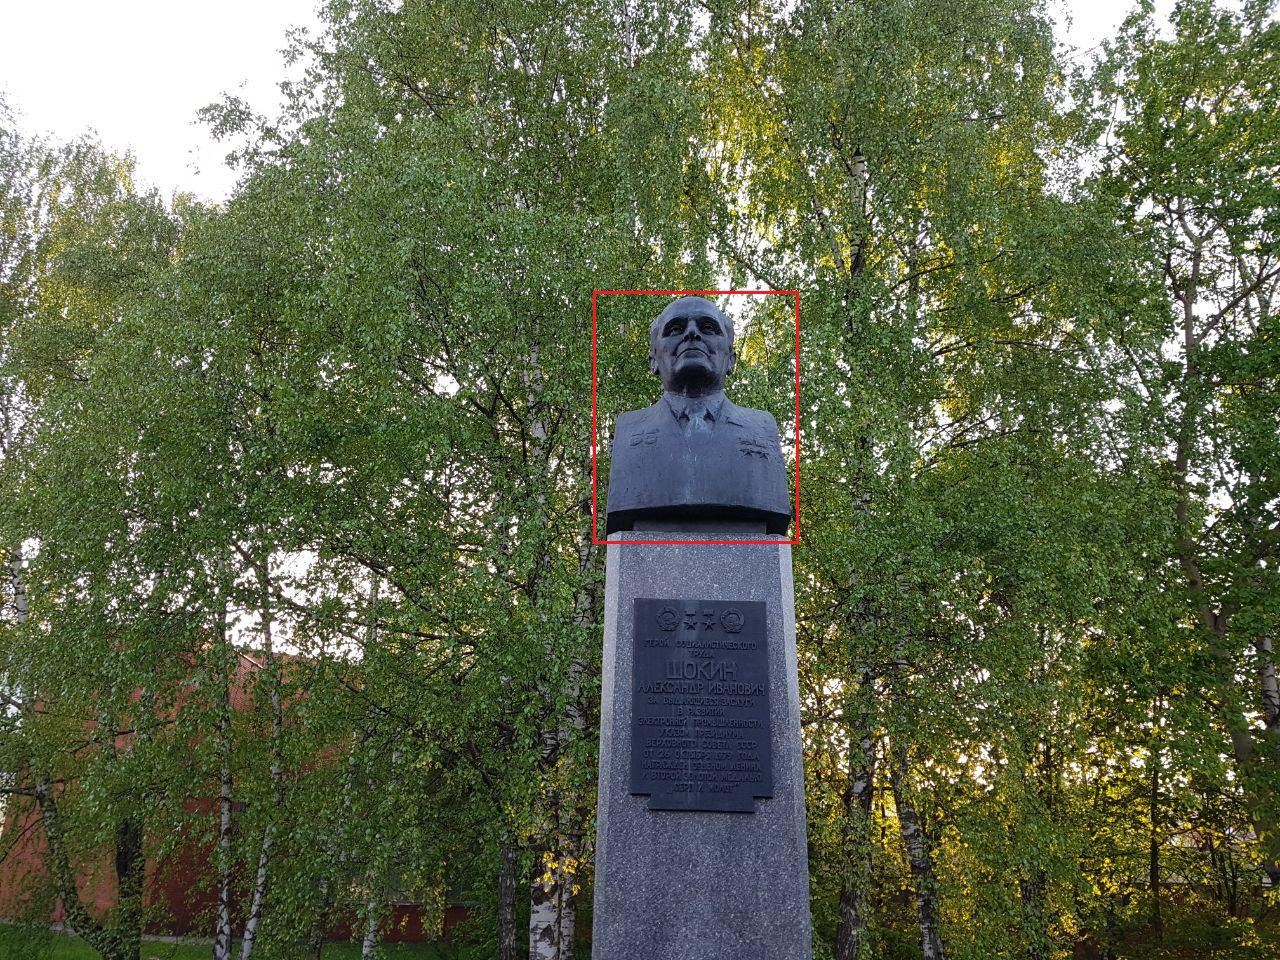
\includegraphics[width=0.49\linewidth]{photo_near}}
		\hfill
		\subbottom[\label{img:photo_far}]{%
			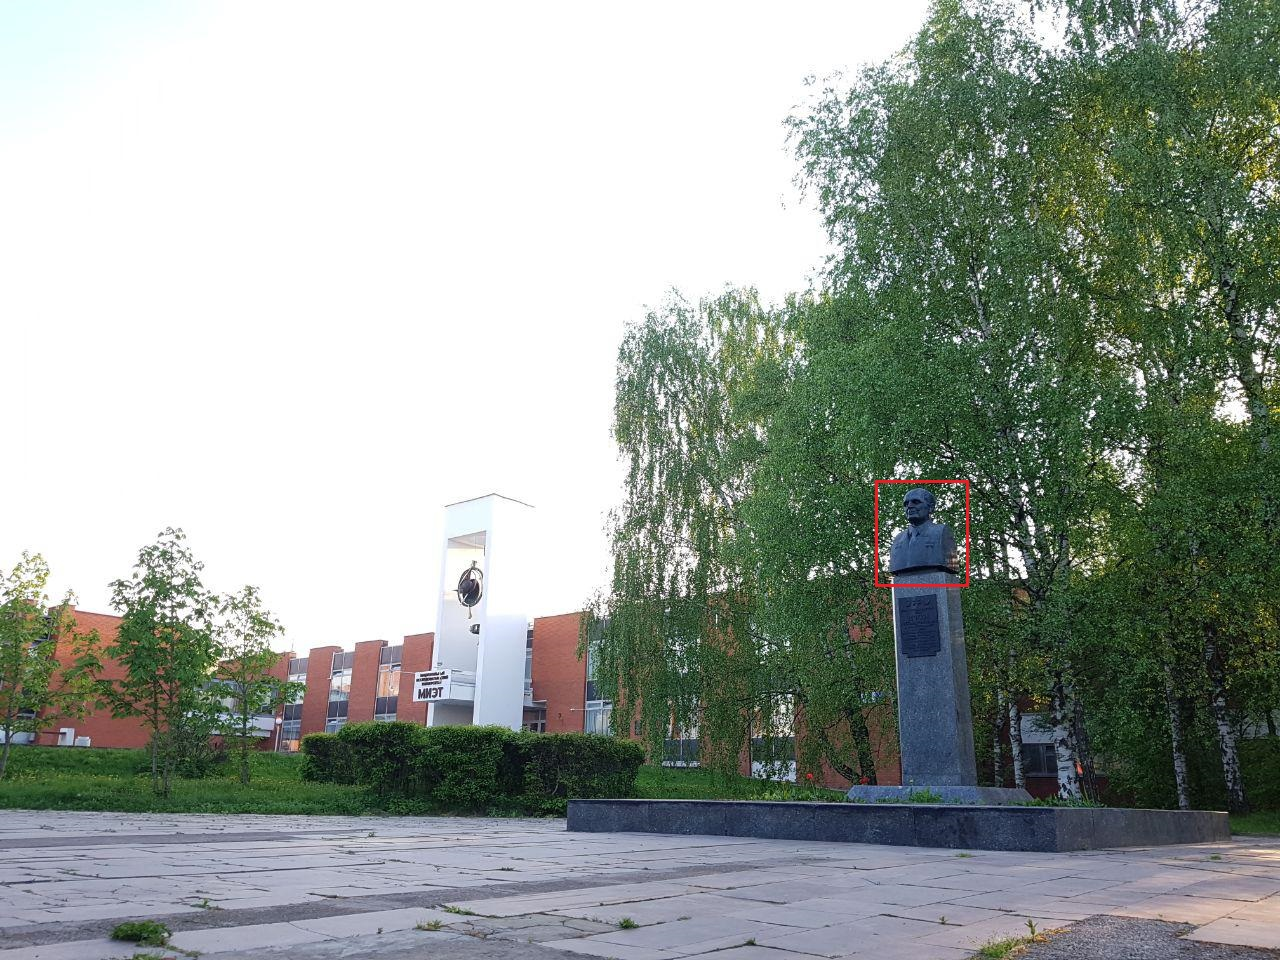
\includegraphics[width=0.49\linewidth]{photo_far}}
		\hfill
	}
	\caption{Пример объекта, сфотографированного с разных ракурсов}
	\label{img:photos}
\end{figure}

\subsection{Базовые примеры дескрипторов}

Как было сказано дескрипторы могут быть самыми разными. Приведем несколько примеров параметров, на которых основывается построения дескриптора~\cite{wiki2017descriptor}:
\begin{enumerate}
	\item Цвет. Это самое базовое качество любого изображения. Существуют множество параметров, которые можно получить из цветов. Примером могут служить:
	\begin{itemize}
		\item Dominant Color Descriptor (DCD);
		\item Color Layout Descriptor (CLD);
		\item Group of Frame (GoF).
	\end{itemize}
	\item Текстура. Также очень важный параметр, описывающий изображения. Дескрипторы на основе текстуры показывают однородность, гистограммы границ области. Примером могут служить:
	\begin{itemize}
		\item Homogeneous Texture Descriptor (HTD);
		\item Texture Browsing Descriptor (TBD);
		\item Edge Histogram Descriptor (EHD).
	\end{itemize}
	\item Форма. Этот параметр содержит очень важную информацию, так как человеческий глаз приспособлен распознавать объекты на основе формы. Однако эту информацию можно извлечь только с помощью сегментации, аналогичной той, которую реализует человеческая визуальная система. В настоящее время такая система ещё недоступна, но существуют неплохие аппроксимации. Примером могут служить:
	\begin{itemize}
		\item Region-based Shape Descriptor (RSD);
		\item Contour-based Shape Descriptor (CSD);
		\item 3-D Shape Descriptor (3-D SD).
	\end{itemize}
	\item Движение. Этот параметр может описывать как движение объекта, так и движение камеры. Примером могут служить:
	\begin{itemize}
		\item Motion Activity Descriptor (MAD);
		\item Camera Motion Descriptor (CMD);
		\item Motion Trajectory Descriptor (MTD);
		\item Warping and Parametric Motion Descriptor (WMD and PMD).
	\end{itemize}
\end{enumerate}

Нас больше всего интересуют дескрипторы, которые описывают форму объекта. Примером параметров описывающих форму фигуры могут служить~\cite{morse2000lecture}:
\begin{enumerate}
	\item Площадь "--- число пикселей в объекте.
	\item Периметр "--- число пикселей на границе объекта.
	\item Компактность "--- как плотно объект составлен, считается как $perimeter^2/area$. Самый компактный объект "--- это круг, он имеет компактность $4\pi$. Все остальные фигуры имеют компактность ниже $4\pi$.
	\item Эксцентриситет "--- отношение длины самой большой хорды фигуры к длине максимальной перпендикулярной хорды. Существуют и другие способы определения этого параметра.
	\item Удлинение "--- отношение высоты и ширины повернутого минимального ограничивающего прямоугольника. Другими словами, необходимо поворачивать объект, строя его ограничивающий прямоугольник. Отношение сторон минимального из построенных прямоугольников и будет ответом.
	\item Прямоугольность "--- насколько прямоуголен объект, считается как отношение площади объекта к площади его ограничивающего прямоугольника. Максимальным значением будет 1 для прямоугольника, минимальным в пределе 0 для тонкой линии.
	\item Ориентация "--- общее направление фигуры.
\end{enumerate}

И это лишь самые простые из возможных числовых параметров некоторой формы. В основном были приведены только дескрипторы описывающие область (RSD). Заметим, что не все из предложенных характеристик удовлетворяют устойчивости к изменению масштаба. Например, площадь как количество пикселей явно не сможет нормально описать объект. Чтобы обойти это ограничение создатели дескрипторов часто приводят описываемые объекты к одному масштабу.

Построение выпуклой оболочки необходимо скорее для дескрипторов прямо основанных на ней~\cite{mathew2015content} или для дескрипторов, описывающих границы объекта (CSD), так как границой может быть и выпуклая оболочка. Именно такие дескрипторы будут рассмотрены далее.

\subsection{Статистические моменты}

Форму границы объекта могут помочь описать даже простые статистические моменты, как математическое ожидание, дисперсия, и другие~\cite{gonzalez2012digital}. На рисунке \ref{img:moments} можно видеть, что мы описали некий сегмент границы объекта с помощью 1D функции $g(r)$. Эта функция получается простым поворотом сегмента, пока он не будет горизонтален.

\begin{figure}[H]
	\centering
	\includesvg[width=\linewidth]{moments}
	\caption{Перевод границы сегмента объекта в одномерную функцию}
	\label{img:moments}
\end{figure}

Теперь необходимо нормализовать $g(r)$ с помощью пложщади сегмента и считать эту функцию "--- гистограмой. Другими словами $g(r_i)$ считается вероятностью значения $r$. Таким образом мы получим формулу момента $n$ на формуле~\eqref{eq:nth_moment}~\cite{gonzalez2012digital}.

\begin{equation}\label{eq:nth_moment}
\mu_n(r)=\sum_{i=0}^{K-1}(r_i "--- m)^n g(r_i)
\end{equation}
где
\begin{equation}\label{eq:mean}
m=\sum_{i=0}^{K-1}r_i g(r_i)
\end{equation}

В этой формуле $K$ "--- это количество точек на границе сегмента. Обычно, чтобы различать формы объектов, хватает первых нескольких моментов. Заметим, что второй момент $\mu_2(r)$ показывает разброс сегмента от среднего, а третий $\mu_3(r)$ измеряет симметричность относительно центра~\cite{gonzalez2012digital}.

Таким образом, мы получили сведение задачи описания двумерной границы объекта к одномерной функции $g$. Преимущество статистических моментов, как дескрипторов объектов "--- это конечно простота имплементации и их понятный физический смысл. Инвариантность к повороту данного метода очевидна. Независимость дескриптора от масштаба может быть достигнута с помощью изменения отрезка значений $g$ и $r$~\cite{gonzalez2012digital}.

Хотя моменты "--- это самый известный и используемый метод, он не единственный, который люди используют часто. Например, Фурье дескрипторы, которые будут объяснены ниже, очень часто помогают описывать форму ещё лучше. 

\subsection{Фурье дескрипторы}

Одним из самых популярных дескрипторов объектов на изображении являются Фурье дескрипторы. Нам они особенно интересны, потому что описывают границу объекта.

Так как мы имеем дело с изображением, то можно каждый пиксель представляет из себя пару координат $(x, y)$. Это даёт возможность рассматривать точки на изображении как комплексные числа $f(k) = x(k) + iy(k), k = 0,1,...,N-1$~\cite{kolyuchkin2013visionAlgorithms}. Таким образом, $x$ "--- это действительная часть, а $y$ "--- это мнимая часть комплексного числа.

По сути мы свели двумерную задачу к одномерной, что даёт нам использовать дискретное преобразование Фурье \eqref{eq:fourierDiscrete} для массива $f(k)$.

\begin{equation}\label{eq:fourierDiscrete}
F(u) = 1/N \sum_{k=0}^{N-1} f(k) \exp(- 2\pi u k / N), u = 0,1,...,N-1
\end{equation}

Комплексные коэффициенты $F(u)$ называются фурье-дескрипторами границы. Вектор признаков формируется $F(u)$ с положительными и отрицательными индексами $u = \pm 1 ,\pm 2, ..., \pm L/2$ причём $L \leq N-1$~\cite{kolyuchkin2013visionAlgorithms}.

Что насчёт инвариантности этого дескриптора? К сожалению этот дескриптор в таком виде хоть и простой, но зависим как от масштаба, так и от перемещения. Чтобы комплексные числа были независимы от перемещения, $f(k)$ считаются с учётом некоего центра $g=(x_g,y_g)$ объекта, чаще всего это центр тяжести точек~\eqref{eq:descriptorCenter}~\cite{thang2010fourier}.

\begin{equation}\label{eq:descriptorCenter}
f(k)=(x(k)-x_g)+i(y(k)-y_g)
\end{equation}

Инвариантность относительно масштаба объекта достигается с помощью нормировки дескрипторов на модуль дескриптора с индексом $u=1$. Тогда вектор признаков примет вид~\cite{kolyuchkin2013visionAlgorithms}:

\[
X=\left(\frac{\lvert{F_{-L/2}}\rvert}{\lvert{F_1}\rvert},...,\frac{\lvert{F_{-2}}\rvert}{\lvert{F_1}\rvert},\frac{\lvert{F_2}\rvert}{\lvert{F_1}\rvert},...,\frac{\lvert{F_{L/2}}\rvert}{\lvert{F_1}\rvert}\right)^T
\]

Значение параметра $L$ определяет размерность признакового пространства $K=L-2$~\cite{kolyuchkin2013visionAlgorithms}.

\subsection{Дерево вогнутости области}

До сих пор были описаны методы, которые могут быть использованы как к самой границе объекта, так и к его выпуклой оболочке, но существуют алгоритмы, которые прямо полагаются на выпуклую оболочку объекта. Один из таких алгоритмов "--- это дерево вогнутости области. Оно генерируется рекурсивно при построении выпуклой оболочки.

Рассмотрим процесс генерации дерева по шагам~\cite{sonka2014image}:
\begin{enumerate}
	\item Строится выпуклая оболочка текущей рассматриваемой фигуры, это показано на рисунке~\ref{img:concavity_tree_1_1}.
	\item Для вогнутых остатков опять строится выпуклая оболочка. На рисунке~\ref{img:concavity_tree_1_2} показано построение оболочки для части $S_2$, которая была выделена после первого шага.
	\item Процесс аналогичным образом продолжается, пока не останется ни одной выгнутой части. Окончательное разбиение показано на рисунке~\ref{img:concavity_tree_2_1}.
	\item В конце работы алгоритма строится дерево, которое показано на рисунке~\ref{img:concavity_tree_2_2}.
\end{enumerate}

\begin{figure}
	{\centering
		\hfill
		\subbottom[\label{img:concavity_tree_1_1}]{%
			\includesvg[width=0.49\linewidth]{concavity_tree_1}}
		\hfill
		\subbottom[\label{img:concavity_tree_1_2}]{%
			\includesvg[width=0.49\linewidth]{concavity_tree_2}}
		\hfill
	}
	\caption{Построение выпуклых оболочек для дерева вогнутости области}
	\label{img:concavity_tree_1}
\end{figure}

\begin{figure}
	{\centering
		\hfill
		\subbottom[\label{img:concavity_tree_2_1}]{%
			\includesvg[width=0.49\linewidth]{concavity_tree_3}}
		\hfill
		\subbottom[\label{img:concavity_tree_2_2}]{%
			\includesvg[width=0.49\linewidth]{concavity_tree_4}}
		\hfill
	}
	\caption{Дерево вогнутости области}
	\label{img:concavity_tree_2}
\end{figure}

Заметим, что граф "--- это хорошо исследованный математический объект, который может служить отличной основой для вычисления дескриптора.

Преимущества такого представления в виде графа очевидны:
\begin{itemize}
	\item инвариантность к любому повороту, переносу или масштабированию;
	\item нечувствительность к небольшим изменениям формы;
	\item гибкость представления позволяет включать в него самые разные характеристики, которые нужны для конкретного применения на практике, например, положение, площадь и поворот;
\end{itemize}

\subsection{Применение выпуклой оболочки}

Как было показано бывают дескрипторы, которые используются в основном для описания границ. Также существует и совершенно другие алгоритмы, которые принципиально работают на основе выпуклых оболочек. Исследователи уже давно используют выпуклые оболочки для того, чтобы считать дескрипторы объектов на изображении~\cite{dalitz2013fourier, mathew2015content, sonka2014image}.

Обычные алгоритмы расчёта дескрипторов, которые основаны на границе объекта, могут быть использованы для описания выпуклой оболочки. Более того, то, где находятся точки на выпуклой оболочке показывает форму объекта, что показано на рисунке \ref{img:alpha_convex_hull}. Как видно в некоторых местах точек больше, в некоторых меньше, это показывает, что слева снизу объект является выпуклым, когда же слева сверху, он вогнутый. Заметим, что именно это свойство используется для построения дерева вогнутости области, но и в обычных алгоритмах это вполне описывают форму объекта.

\begin{figure}[H]
	\centering
	\includesvg[scale=0.5]{alpha_convex_hull}
	\caption{Точки выпуклой оболочки символа альфа}
	\label{img:alpha_convex_hull}
\end{figure}

\section{Анализ текущего состояния алгоритмов и выявление проблемы} \label{sect1_2}

Как было сказано, выпуклые оболочки могут легко использоваться для того, чтобы описывать объекты на изображении. И надо заметить, что очень часто вычисления происходят в реальном времени, например, обработка видео-потока с камеры. Для того, чтобы быстро вычислять дескрипторы, нужны быстрые алгоритмы. Причём они должны использоваться в каждой части вычисления.

Эта работа прежде всего сконцентрирована на оптимизации части вычисления выпуклой оболочки объекта.

Почему же нас не устраивают все те алгоритмы, которые давно уже были придуманы? Есть несколько причин. Рассмотрим самый быстрый, судя по сложности алгоритма, алгоритм Чана. Алгоритм Чана хоть и является оптимальным по сложности, всё же уступает другим алгоритмам в константе, которая скрывается за этой сложностью. У алгоритма множество этапов, и он явно проигрывает по времени работы остальным алгоритмам. На это явно указывает его отстуствие во всех популярных библиотеках для компьютерного зрения: OpenCV~\cite{opencvconvexhull}, CGAL~\cite{cgalconvexhull}, QHull~\cite{qhull} и другие.

Но какой алгоритм тогда используется? Используется алгоритм Грэхема и другие алгоритмы за $O(n \log n)$. Хоть он и не является оптимальным он самый быстрый, потому что сортировка (самый долгий этап алгоритма) уже давно оптимизирована и написана настолько хорошо, что константа становится очень маленькой.

Именно в этом и заключается проблема. С одной стороны есть оптимальный с точки зрения сложности алгоритм, который не используется, а с другой алгоритм, не являющийся оптимальным, но активно применяющийся на практике.

Асимптотика числа вершин выпуклой оболочки для $n$ точек явно показывает, что преобладает малое количество точек в итоговой выпуклой оболочке:
\begin{itemize}
	\item при равномерном распределении внутри круга "--- $\theta( n^{1/3} )$;
	\item при равномерном распределении внутри фиксированного выпуклого многоугольника "--- $\theta(\log n)$;
	\item при двумерном нормальном распределении "--- $\theta((\log n)^{1/2})$~\cite{algolist2010convexhull}.
\end{itemize}

Получается, что для малого набора точек в итоговой выпуклой оболочке мы имеем время работы, которое явно можно улучшить.

\section{Выводы} \label{subsect1_4}

В результате исследования можно с уверенностью сказать, что построение выпуклых оболочек является очень важной частью описания объектов на изображении. Мы привели множество таких методов вычисления дескрипторов.

После рассмотрения популярных существующих решений построения выпуклых оболочек и анализа состояния проблемы, можно с уверенностью сказать, что необходимо пересмотреть этап построения выпуклой оболочки и сделать его более эффективным.

Необходимо разработать алгоритм, хорошо работающий на множествах точек, из которых только малое количество реально будет в итоговой выпуклой оболочке, как это и бывает на практике. Это прежде всего означает, что алгоритм должен иметь сложность $O(n \log{h})$ в среднем случае, что позволит ему быть лучше, чем популярные в данный момент алгоритмы со сложностью $O(n \log{n})$.

Также необходимо не забывать о применении этого алгоритма, он будет использоваться в первую очередь для построения выпуклых оболочек с последующим вычислением дескриптора объекта, для которого мы и строили оболочку. Если можно получить некую дополнительную информацию об объекте, то это выгодно отличит наш алгоритм в сравнении с самым популярным алгоритмом Грэхема.

           % Глава 1
\chapter{Разработка нового алгоритма построения выпуклой оболочки} \label{chapt2}

\section{Формализация понятия выпуклой оболочки} \label{sect2_1}

Формализация задачи "--- это очень важная часть любого исследования, которая позволяет правильно анализировать результаты работы. Итак, чтобы разработать алгоритм построения выпуклой оболочки конечного множества точек на плоскости, необходимо формализовать данное понятие.

Пусть дано множество $S$ точек. Выпуклой оболочкой данного множества называется наименьшее выпуклое множество, содержащее $S$. Формально выпуклая оболочка может быть определена как пересечение всех выпуклых множеств, которые содержат $S$.

Это определение является самым популярным и общим, но оно слишком далеко от практики, поэтому мы будем использовать другое. Заметим, что разрабатываемый алгоритм должен работать только для плоскости, поэтому мы будем использовать определение, которое работает только для случая двумерного пространства.

Для формализации понятия выпуклой оболочки, нам снова понадобится предикат $ccw$, описанный в формуле \eqref{eq:ccw}. Выпуклой оболочкой множества $S$ будет называться выпуклый многоугольник $T$ с вершинами $t_i \in S$, пронумерованными против часовой стрелки для $i = 1,...,n$~\cite{pichardie2001formalizing}. Причём обязательно выполнения условия \eqref{eq:convex_hull_def}.

\begin{equation}\label{eq:convex_hull_def}
\forall [t_i, t_{i+1}] \in T, p \in S \backslash \{ t_i, t_{i+1} \} : ccw(t_i, t_{i+1}, p)
\end{equation}

Это выражение утверждает, что каждая точка $p$, принадлежащая $S$, кроме текущего ребра $t_i, t_{i+1}]$, находится слева от него. Это свойство выпуклой оболочки отлично показано на рисунке \ref{img:convex_hull_def} с помощью ориентированных рёбер. Видно, точек справа от ребра нет, иначе бы это ребро не принадлежало выпуклой оболочке.

\begin{figure}[hbt]
	{\centering
		\hfill
		\subbottom[Конечное множество точек $S$\label{img:convex_hull_def_1}]{%
			\includesvg[width=0.45\linewidth]{convex_hull_def_1}}
		\hfill
		\subbottom[Выпуклая оболочка с ориентированными рёбрами\label{img:convex_hull_def_2}]{%
			\includesvg[width=0.45\linewidth]{convex_hull_def_2}}
		\hfill
	}
	\caption{Формализация понятия выпуклой оболочки}
	\label{img:convex_hull_def}
\end{figure}

Заметим, что это определение никак не нарушает требование минимальности выбранного многоугольника, так как мы составляем выпуклую оболочку из точек, которые принадлежат множеству $S$.

\section{Описание алгоритма основанного на использовании бинарного дерева} \label{sect2_2}

\subsection{Основная идея} \label{subsect2_2_1}

Основная идея предлагаемого в данной работе алгоритма очень похожа на принцип, лежащий в основе инкрементального алгоритма, уже рассмотренного выше. Мы можем хранить точки в сбалансированном по высоте двоичном дереве поиска. Точки в инкрементальном алгоритме хранились в верхнем и нижнем деревьях и были отсортированы по координате $x$. Мы будем использовать другой подход, который позволит хранить точки только в одном дереве, узлы (точки) будут отсортированы по углу относительно приблизительного центра выпуклой оболочки.

Чтобы объяснить работу алгоритма нам понадобится уже известный нам предикат $ccw$, определённый в формуле \eqref{eq:ccw} и понятие экстремальной точки.

Экстремальная точка множества $S$ "--- это точка, которая точно принадлежит выпуклой оболочке $S$. Обычно это точка, которая лежит дальше от всех по какому либо параметру. Например, самая левая или верхняя точка точно будет входить в итоговую выпуклую оболочку.

Пусть дано множество точек $S$ и необходимо найти выпуклую оболочку данного множества.

Первый шаг алгоритма "--- это нахождение приближенного центра, с помощью которого будут отсортированы в дереве точки. Хорошей аппроксимацией центра для наших целей будет среднее арифметическое трёх экстремальных точек:
\begin{itemize}
	\item левая крайняя точка $A$;
	\item правая крайняя точка $B$;
	\item точка $C$, которая наиболее удалена от линии $A,B$.
\end{itemize}

На рисунке~\ref{img:my_extreme_points_1} показан пример, найденных на первом шаге алгоритма, экстремальных точек. Потом на рисунке~\ref{img:my_extreme_points_2} находится точка $D$ "--- это приближённый центр выпуклой оболочки, который мы искали. После нахождения центра мы добавляем точки $A, B, C$ в наше дерево поиска.

\begin{figure}[hbt]
	{\centering
		\hfill
		\subbottom[\label{img:my_extreme_points_1}]{%
			\includesvg[width=0.45\linewidth]{my_extreme_points_1}}
		\hfill
		\subbottom[\label{img:my_extreme_points_2}]{%
			\includesvg[width=0.45\linewidth]{my_extreme_points_2}}
		\hfill
	}
	\caption{Нахождение приближённого центра выпуклой оболочки}
	\label{img:my_extreme_points}
\end{figure}

Остальные точки будут добавлены в случайном порядке. Рассмотрим процесс добавления очередной точки в текущую выпуклую оболочку множества.

Пусть мы уже построили дерево поиска, в котором содержится наша выпуклая оболочка, отсортированная по углу относительно центра $D$, найденного ранее. Теперь необходимо добавить новую точку $A$.

Первое, что необходимо найти "--- это две точки $L$ и $R$. Точки $L$, $R$ "--- это точки слева и справа соответственно от $A$ по углу относительно центра $D$. Как видно на рисунке \ref{img:my_find_lr}, все точки хранятся по углу относительно точки $D$, и поэтому поиск точек не вызывает труда.

\begin{figure}[hbt]
	\centering
	\includesvg[width=\linewidth]{my_find_lr}
	\caption{Нахождение точек $L, R$ в бинарном дереве поиска}
	\label{img:my_find_lr}
\end{figure}

Заметим, что может так оказаться, что точки $L$ и $R$ окажутся в противоположных частях бинарного дерева поиска. Это показано на рисунке \ref{img:my_find_cyclic}. Поэтому мы будем считать, что наше используемое сбалансированное двоичное дерево поиска является цикличным. Заметим, что для этого не требуется никаких специальных дополнительных структур данных. Всё, что нужно делать "--- это при обходе дерева и достижении последней точки, переходить на первую.

\begin{figure}[hbt]
	\centering
	\includesvg[width=\linewidth]{my_find_cyclic}
	\caption{Демонстрация цикличности используемого дерева поиска}
	\label{img:my_find_cyclic}
\end{figure}

После чего может быть 2 случая. Если $ccw(L, R, A)$ не выполняется, то новая точка $A$ не должна быть частью выпуклой оболочки и может быть пропущена. Этот случай показан на рисунке~\ref{img:my_point_cases_1}. Иначе $A$ должна быть частью выпуклой оболочки и мы продолжим добавлять её. Это показано на рисунке~\ref{img:my_point_cases_2}.

\begin{figure}[hbt]
	{\centering
		\hfill
		\subbottom[\label{img:my_point_cases_1}]{%
			\includesvg[width=0.49\linewidth]{my_add_point_1}}
		\hfill
		\subbottom[\label{img:my_point_cases_2}]{%
			\includesvg[width=0.49\linewidth]{my_add_point_2}}
		\hfill
	}
	\caption{Добавление новой точки в выпуклую оболочку}
	\label{img:my_point_cases}
\end{figure}

Итак, мы определили, что точка $A$ должна быть на выпуклой оболочке. Теперь необходимо удалить точки, которые будут внутри оболочки после добавления точки $A$. Это делается с помощью итерации по точкам вправо (аналогичный алгоритм должен быть выполнен для левой стороны) от новой точки. Чтобы определить должна ли точка быть удалена или нет мы будем использовать подход, похожий на тот, который используется в алгоритме Грэхема. Каждые два смежных ребра выпуклой оболочки должны лежать против часовой стрелки.

Пусть следующая точка, которая рассматривается на удаление "--- это $B$. Рассмотрим процесс удаления точки $B$.
\begin{enumerate}
	\item Назовем точку, которая идет следующей после $B$, $C$.
	\item Если $ccw(C, B, A)$ тогда $B$ не должна быть удалена и мы должны прекратить удаление точек в эту сторону, потому что все точки после $B$ уже удовлетворяют условию выпуклой оболочки. По сути этот предикат и проверяет условие лежания смежных ребер против часовой стрелки, о котором говорилось ранее.
	\item Иначе точка $B$ должны быть удалена, так как она оказалась внутри новой выпуклой оболочки.
	\item После чего необходимо рассмотреть точку $C$ как следующего кандидата на удаление и перейти к шагу 1.
\end{enumerate}

На рисунках \ref{img:my_points_deletion_1_1} и \ref{img:my_points_deletion_1_2} можно видеть, что точки $C, B, A$ лежат по часовой стрелке, поэтому точка $B$ должна быть удалена из выпуклой оболочки. Рисунок \ref{img:my_points_deletion_2_1} демонстрирует, что мы должна прекратить удаление точек справа от новой точки, так как $C, B, A$ теперь формирует тройку, которая лежит против часовой стрелки. Аналогично удаление не нужно производить слева от точки, что показано на рисунке \ref{img:my_points_deletion_2_2}. Действительно, на рисунках видно, что в конце получилась готовая выпуклая оболочка добавленных на текущий момент точек.

\begin{figure}[hbt]
	{\centering
		\hfill
		\subbottom[\label{img:my_points_deletion_1_1}]{%
			\includesvg[width=0.49\linewidth]{my_add_point_3}}
		\hfill
		\subbottom[\label{img:my_points_deletion_1_2}]{%
			\includesvg[width=0.49\linewidth]{my_add_point_4}}
		\hfill
	}
	\caption{Удаление точек, которые оказались внутри выпуклой оболочки}
	\label{img:my_points_deletion_1}
\end{figure}

\begin{figure}[hbt]
	{\centering
		\hfill
		\subbottom[\label{img:my_points_deletion_2_1}]{%
			\includesvg[width=0.49\linewidth]{my_add_point_5}}
		\hfill
		\subbottom[\label{img:my_points_deletion_2_2}]{%
			\includesvg[width=0.49\linewidth]{my_add_point_6}}
		\hfill
	}
	\caption{Критерий завершения удаления точек}
	\label{img:my_points_deletion_2}
\end{figure}

Как видно этот процесс очень схож с процессом добавления точек в инкрементальном алгоритме. Существуют такие небольшие различия, как одно дерево вместо двух, цикличность этого дерева, отсутствие граничного случая на стыке двух деревьев и т.д. Они хоть и небольшие, но позволяют алгоритму быстрее добавлять точки в выпуклую оболочку.

Блок-схема всего алгоритма показана на рисунках \ref{img:my_algo} и \ref{img:my_algo_deletion}.

\begin{figure}
	\centering
	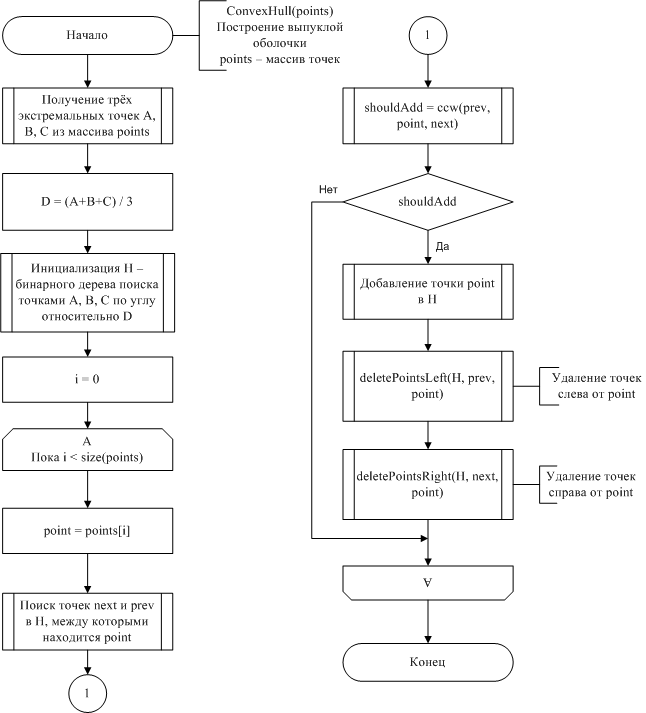
\includegraphics[width=\linewidth]{my_algo}
	\caption{Блок-схема работы предлагаемого алгоритма}
	\label{img:my_algo}
\end{figure}

\begin{figure}
	\centering
	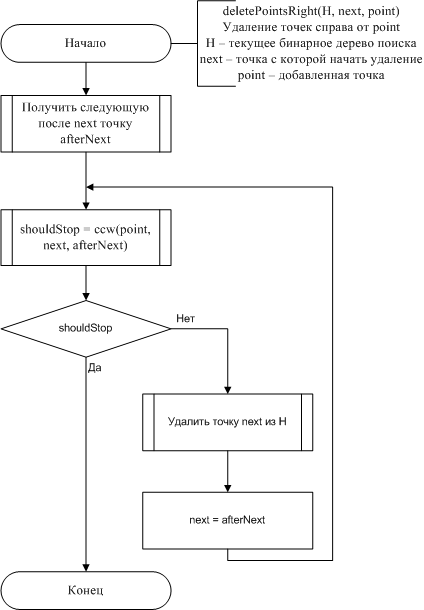
\includegraphics[width=0.7\linewidth]{my_algo_2}
	\caption{Блок-схема функции удаления точек перед добавлением точки point}
	\label{img:my_algo_deletion}
\end{figure}

\subsection{Детали реализации} \label{subsect2_2_2}

Первая важная деталь, которая упрощает реализацию нашего алгоритма "--- это конечно преобразование точек. Намного удобнее считать, что приближённый центр $D$, получение которого описывалось в предыдущей главе "--- это точка $0, 0)$. Как показано в \eqref{eq:ccw} мы вычисляем $ccw$ через $det$, а вычислять $det(A, B, D)$ легче, если $D_x = 0$ и $D_y = 0$. Также нельзя забывать про конечную цель вычисления выпуклой оболочки. Для вычисления дескриптора опять намного удобнее пользоваться координатами уже переведёнными в центр объекта, так как на дескриптор никак не должно влиять положения объекта на изображении.

Вторая деталь, которая также важна при реализации "--- это углы относительно центра, про которые мы так много говорили. Вычисление углов через тригонометрические операции "--- это очень долго, и в этом случае наш алгоритм не смог бы конкурировать по производительности с самыми популярными алгоритмами вычисления выпуклой оболочки.

Необходимо придумать предикат, который бы определял положение точек в дереве, которое хранит текущую выпуклую оболочку. Первой попыткой придумать такой предикат будет использование предиката $ccw$, как это показано в \eqref{eq:my_ccw_predicate}.

\begin{equation}\label{eq:my_ccw_predicate}
A<B=ccw(A, B, (0, 0))
\end{equation}

Заметим, что можно использовать точку $(0, 0)$ как центр, так как точки $A, B$ уже преобразованы в новую систему координат.

К сожалению, такой предикат не соответствует strict weak ordering~\cite{isoCppStd2017}, потому что не выполняется транзитивность. Как можно видеть на рисунке \ref{img:non_transitivity_1} выполняется $ccw(A, B, D)$, поэтому $A$ меньше $B$. При этом выполняется $ccw(B, C, D)$, поэтому $B$ меньше $C$. Но на рисунке \ref{img:non_transitivity_2} в это еже время показано, что не выполняется $ccw(A, C, D)$, то есть $A$ не меньше $C$. В итоге имеем $A < B < C <= A$, что, очевидно, неверно.

\begin{figure}[hbt]
	{\centering
		\hfill
		\subbottom[\label{img:non_transitivity_1}]{%
			\includesvg[width=0.45\linewidth]{non_transitivity_1}}
		\hfill
		\subbottom[\label{img:non_transitivity_2}]{%
			\includesvg[width=0.45\linewidth]{non_transitivity_2}}
		\hfill
	}
	\caption{Нетранзитивный предикат}
	\label{img:non_transitivity}
\end{figure}

Итак, необходимо сделать такую функцию, которая принимает точки $A$ и $B$ и возвращает $true$, если $A$ меньше $B$, иначе $false$. Эта функция будет использована в сбалансированном дереве поиска как компаратор. Был использован следующий алгоритм:

\begin{algorithm}[H]
	\caption{BSTPredicate "--- компаратор для сравнения точек}
	\label{alg:bst_predicate}
	\begin{algorithmic}[1]
		\Procedure{BSTPredicate}{$A, B$}
		\State $leftUp \gets 0<y_A$
		\State $rightUp \gets 0<y_B$
		\If {$leftUp \neq rightUp$}
			\Return $leftUp < rightUp$
		\EndIf
		\If {$(y_A=0) \& (y_B=0)$}
			\Return $(0<x_A) < (0<x_B)$
		\EndIf
		\Return $ccw(A, B, (0, 0))$
		\EndProcedure
	\end{algorithmic}
\end{algorithm}

Эта несложная функция реализует корректный для сортировки предикат. Для этого изначально она делит всю плоскость координат на две части: верхнюю и нижнюю. Как мы видим предикат принимает 2 точки $A$ и $B$. Рассмотрим три случая:
\begin{enumerate}
	\item Если эти точки лежат на разных сторонах. Например, точка $A$ лежит ниже точки $B$, тогда предикат вернет $true$, что будет означать, что $A$ меньше $B$.
	\item Граничный случай, когда обе точки находятся на оси $x$. Тогда нужно определить с какой стороны от оси $y$ они находятся. Если с одной, то токи равны, потому что угол до них одинаков. Иначе меньше точка, которая находится слева.
	\item Если точки находятся в одной полуплоскости, то предикат $ccw$, показанный в формуле \eqref{eq:ccw}, отлично справляется со своей задачей.
\end{enumerate}

Пример порядка точек, вычисленного, с помощью алгоритма BSTPredicate показан на рисунке \ref{img:BSTPred_ordering}.

\begin{figure}[hbt]
	\centering
	\includesvg{BSTPred_ordering}
	\caption{Сортировка точек предикатом BSTPredicate}
	\label{img:BSTPred_ordering}
\end{figure}

\section{Доказательство корректности работы алгоритма} \label{subsect2_3}

Доказательство корректности работы алгоритма удобнее всего построить с помощью математической индукции.

Базис индукции "--- это 3 изначально добавленные в выпуклую оболочку точки. Необходимо доказать, что в начальном шаге выпуклая оболочка удовлетворяет условию \eqref{eq:convex_hull_def}.

Любые 3 точки, не лежащие на одной прямой, являются выпуклой оболочкой, так как они формируют треугольник. Единственное условие, которое необходимо соблюсти "--- это правильный порядок этих точек. Это условие обеспечивается бинарным деревом поиска с предикатом BSTPredicate, поэтому первые три точки являются выпуклой оболочкой.

Пусть теперь для $N$ рассмотренных точек была построена валидная выпуклая оболочка и сейчас рассматривается точка $p_{N+1}$. Как описано выше, при добавление точки необходимо рассматривать два варианта.

Если точка оказалась внутри выпуклой оболочки, то она не может быть добавлена. Заметим, если точка внутри выпуклого многоугольника, то она находится справа от любого его ребра. Этот случай уже был показан на рисунке \ref{img:convex_hull_def_2}. Очевидно, что если точка не добавляется и до этого выпуклая оболочка была правильно построена, то и после она будет валидна.

Второй случай является более сложным. Точка должна быть добавлена в существующую выпуклую оболочку. Процесс удаление точек уже был показан на рисунке \ref{img:my_points_deletion_1}. Важное в этом процессе, что он делается по критерию не выполнения $ccw(C, B, A)$, что абсолютно идентично критерию выпуклой оболочки в формуле \eqref{eq:convex_hull_def}. На рисунке \ref{img:my_proof_1} показано выполнение условия выпуклой оболочки для новой добавленной точки. Из-за условия удаления точно известно, что после добавления новой точки $p_{N+1}$ удалённые точки и точки $C_1, C_2$ находятся слева от новых рёбер $p_{N+1}, A$ и $B, p_{N+1}$. Осталось показать, что остальные точки также лежат левее этих рёбер.

\begin{figure}[hbt]
	\centering
	\includesvg{my_proof_1}
	\caption{Состояние выпуклой оболочки после добавления новой точки}
	\label{img:my_proof_1}
\end{figure}

Предположим, что существует такая точка $k$, что она лежит правее новых ребер. Заметим, что эта точка может лежать только левее прямой $B, A$, так как все точки правее были рассмотрены в процессе удаления. Также заметим, что было показано, что выполняются предикаты $ccw(p_{N+1}, A, C_2)$ и $ccw(C_1, A, p_{N+1})$. В это же время для ребер $A, C_2$ и $C_1, B$ по предположению индукции мы знаем, что все точки лежат левее их. Получаем противоречие, потому что точка $k$ должна лежать правее новых рёбер, но при этом она должна лежать левее линий $C_1, B$; $B, A$; $A, C_2$. На изображении~\ref{img:my_proof_2} отлично видно, что две эти области не пересекаются. Таким образом, корректность выпуклой оболочки после добавления новой точки сохраняется.

\begin{figure}[hbt]
	\centering
	\includesvg{my_proof_2}
	\caption{Области, где может лежать точка}
	\label{img:my_proof_2}
\end{figure}

\section{Оценка сложности алгоритма} \label{subsect2_4}

Пусть дано множество точек $S$ размера $N$.

Первое, что необходимо определить "--- это временную сложность алгоритма.

На шаге инициализации алгоритма проводиться поиск трёх экстремальных точек. Это делается за $2 N$ шагов, так как надо сначала найти самые левую и правую точки, а потом найти самую дальнюю от них другую точку.

После чего точки рассматриваются в случайном порядке. Изначально необходимо найти положение точки в бинарном дереве. Эта операция делается за $O(\log h)$, где $h$ "--- это текущее количество точек в выпуклой оболочке.

Если эту точку необходимо добавить, то далее удаляются все точки, которые после добавления точки окажутся внутри выпуклой оболочки. Сложность операции удаления точки может варьироваться для разных сбалансированных двоичных деревьев поиска. В стандарте языка C++ сказано, что амортизированная сложность операции удаления из $std::set$ по итератору является $O(1)$~\cite{isoCppStd2017}. Поэтому будем считать, что у операции удаления константная сложность.

Во время работы алгоритма максимальное количество удалений не может превышать $N$, так как всего $N$ точек рассматривается. Поэтому эта операция занимает $O(N)$ времени.

Пусть максимальный размер выпуклой оболочки за время работы алгоритма равен $M$. Тогда сложность поиска точек за всё время работы алгоритма равна $O(N \log M)$.

В итоге сложность алгоритма равна:
\[
O(2 N + N + N \log M) = O(N \log M)
\]

Заметим, что в обычном случае количество точек в дереве будет примерно около $H$ всё время работы алгоритма, что позволяет нам сказать, что средняя сложность будет равняться $O(N \log H)$, где $H$ "--- это количество точек в финальной выпуклой оболочке. Заметим, что так как точки добавляются в случайном порядке, обычно именно такая сложность и будет достигаться. 

Если рассматривать точки не в случайном порядке, то возможно подобрать тесты, при которых сложность алгоритма будет равняться $O(N \log N)$. Поэтому мы считаем, что в худшем случае наш алгоритм будет иметь именно такую временную сложность. 

Сколько памяти потребляет предлагаемый алгоритм? Кроме хранения входных данных предлагаемому в данной работе алгоритму необходимо хранить также сбалансированное двоичное дерево поиска с точками, которые сейчас принадлежат выпуклой оболочке. Поэтому сложность по памяти будет равняться $O(M)$. Аналогично временной сложности средняя равна $O(H)$, когда же в худшем случае это $O(N)$.

\section{Выводы} \label{subsect2_5}

Разработанный в этой главе алгоритм построения выпуклой оболочки имеет множество преимуществ, которые безусловно нужны при выполнении задач компьютерного зрения. Он:
\begin{itemize}
	\item является оптимальным в среднем случае (имеет сложность $O(n \log h)$);
	\item предоставляет дополнительные данные для будущего построения дескриптора (приблизительный центр объекта);
	\item имеет возможность к настройке под конкретные практические нужды с помощью изменения реализации сбалансированного двоичного дерева поиска (AVL, красно-чёрные деревья, и т.д.);
	\item прост в имплементации;
	\item позволяет добавлять точки и после окончания работы алгоритма.
\end{itemize}

Заметим, что требования, которые выдвигались в выводах к первой главе были удовлетворены.

До сих пор обсуждались лишь теоретические выкладки. Следующий шаг "--- это проверка алгоритма на практике.
           % Глава 2
\chapter{Разработка предлагаемого алгоритма и системы сравнения быстродействия алгоритмов построения выпуклых оболочек} \label{chapt3}

\section{Разработка методики сравнения алгоритмов}

\subsection{Минусы классической методики сравнения}

Большинство сравнений алгоритмов построения выпуклой оболочки не зависят от выходных данных. А как было продемонстрировано в предыдущих главах именно от количества точек в финальной выпуклой оболочке зависит время работы многих из них.

Большинство сравнений полагается на некоторые допущения по случайному распределению точек на плоскости. Вот некоторые из них~\cite{chadnov2004algorithmsComparison}:

\begin{enumerate}
	\item Равномерное распределение в единичном квадрате.
	\item Равномерное распределение в единичном круге.
	\item Нормальное распределение в единичном квадрате.
	\item Распределение Лапласа в единичном квадрате с центром распределения в точке $(0.5, 0.5)$.
	\item Равномерное распределение точек на окружности.
\end{enumerate}

%TODO: добавить рисунки разных распределений

Как видно из этого списка, количество точек в финальной выпуклой оболочке будет каким-то фиксированным для каждого из выбранного способа. Например, при распределении внутри единичного круга число вершин в выпуклой оболочке для $n$ точек будет $\theta(n^{1/3})$~\cite{algolist2010convexhull}. А для распределения на окружности очевидно, что количество точек в выпуклой оболочке будет равно изначальному количеству точек.

Такой подход не даёт полноту картины для разного количества точек в выпуклой оболочке. Он привязывает к сравнению всего лишь на основе одного параметра "--- количества точек. Поэтому было решено разработать новую методику сравнения алгоритмов, которая бы давала эту возможность.

\subsection{Идея сравнения на основе выходного параметра алгоритма}

Основная идея, которая будет использоваться при сравнении алгоритмов "--- это мы будем сравнивать не только опираясь на $n$ (изначальное количество точек), но и на $h$ (количество точек в выпуклой оболочке).

Для того, чтобы достичь этого, необходимо придумать способ генерировать тестовые данные с фиксированным процентом точек, которые будут в выпуклой оболочке. Сперва генерация происходит на окружности, эти точки точно будут на выпуклой оболочке. Это показано на рисунке \ref{img:points_gen_1}. После чего необходимо сгенерировать точки, которые будут лежать внутри выпуклой оболочки и не попадут в неё. Это можно сделать с помощью генерации точек внутри круга, что показано на рисунке \ref{img:points_gen_2}. Финальным шагом мы перемешываем эти точки и всё. Входные данные с фиксированным процентом точек на выпуклой оболочке готовы.

\begin{figure}
	{\centering
		\hfill
		\subbottom[\label{img:points_gen_1}]{%
			\includesvg[width=0.45\linewidth]{gen_1}}
		\hfill
		\subbottom[\label{img:points_gen_2}]{%
			\includesvg[width=0.45\linewidth]{gen_2}}
		\hfill
	}
	\caption{Генерирование точек с фиксированным процентом на выпуклой оболочке}
	\label{img:points_gen}
\end{figure}

Проблема генерации точек внутри круга как на рисунке \ref{img:points_gen_2} в том, что эти точки всё равно могут стать выпуклой оболочкой множества. Этот случай показан на рисунке \ref{img:gen_error}. На этом рисунке красные точки слева и справа были сгенерированы внутри круга, но они попали в выпуклую оболочку.

\begin{figure}[H]
	\centering
	\includesvg[width=0.7\linewidth]{gen_error}
	\caption{Ошибка генерации точек внутри выпуклой оболочки}
	\label{img:gen_error}
\end{figure}

Для того, что исправить эту проблему необходимо после генерации точек, которые будут лежать на выпуклой оболочке генерировать остальные точки внутри получившегося многоугольника. Как же это сделать? Для того, чтобы сгенерировать случайную точку внутри многоугольника необходимо разбить его на треугольники, что показано на рисунке \ref{img:triangles}.

\begin{figure}[H]
	\centering
	\includesvg[width=0.7\linewidth]{triangles}
	\caption{Разбиение выпуклого многоугольника на треугольники}
	\label{img:triangles}
\end{figure}

Заметим, что равномерный случайный выбор треугольника не может быть произведён, потому что треугольники имеют разные площади, поэтому выбирать треугольник, в котором будет генерироваться случайная точка необходимо с весами, равными площадям этих треугольников. После чего остается только вычислить случайную точку $P$ внутри треугольника, который составляют точки $A, B, C$. Это можно сделать с помощью формулы~\eqref{eq:randomInTriangle}~\cite{osada2002shape}.

\begin{equation}\label{eq:randomInTriangle}
P = (1 "--- \sqrt{r1}) * A + (\sqrt{r1} * (1 "--- r2)) * B + (\sqrt{r1} * r2) * C
\end{equation}
где $r1, r2$ "--- это равномерно распределённое случайное число в отрезке [0, 1].

\section{Сравнение алгоритмов}

\subsection{Описание используемой библиотеки и параметров сравнения}

Для сравнительного тестирования была выбрана библиотека CGAL, как одна из самых популярных библиотек для вычислительной геометрии. Эта библиотека предоставляет несколько функций для построения выпуклой оболочки~\cite{cgalconvexhull}:
\begin{itemize}
	\item $ch\_akl\_toussaint$ "--- функция, использующая алгоритм Akl-Toussaint~\cite{akl1978fast}, сложность равна $O(n \log n)$;
	\item $ch\_bykat$ "--- функция, использующая алгоритм Eddy~\cite{eddy1977new}, сложность равна $O(nh)$;
	\item $ch\_bykat$ "--- функция, использующая нерекурсивную версию алгоритма Eddy~\cite{bykat1978convex}, сложность равна $O(nh)$;
	\item $ch\_graham\_andrew$ "--- функция, использующая версию Andrew алгоритма Грэхема~\cite{andrew1979another}, сложность равна $O(n \log n)$;
	\item $ch\_jarvis$ "--- функция, использующая алгоритм Джарвиса~\cite{jarvis1973Jarvis}, сложность равна $O(nh)$.
\end{itemize}

Как видно всего 2 алгоритма имеют сложность $O(n \log h)$. Мы будем проводить сравнение с алгоритмом Грэхема как с самым популярным из предложенных.

Программа, которая используется для сравнения алгоритмов лежит в свободном доступе~\cite{matrokhin2017github} и включает в себя 2 модуля:
\begin{enumerate}
	\item Написанный на C++ первый модуль включает в себя запуск и замер времени работы алгоритмов построения выпуклой оболочки. Оболочка строится для множества точек, которые были записаны в файл. Также этот модуль включает имплементацию разработанного в данной работе алгоритма.
	\item Написанный на Python второй модуль включает в себя прежде всего генерацию изначального множества точек, удовлетворяющим условия тестирования, и запуск программы для этих данных. После запуска строятся графики и выводятся табличные данные по полученным результатам.
\end{enumerate}

Для сравнения алгоритмов использовался среднестатистический компьютер. Тем не менее, понятно, что всё это можно повторить и на любых других системах.

Ниже приведены параметры системы, на которой проводилось сравнение:
\begin{enumerate}
	\item Процессор: Intel Core i5-6600K
	\item Оперативная память: Kingston HyperX FURY Black DDR4 2666MHz 8GB
	\item Операционная система: Windows 10 (Version 1803)
	\item Компилятор: C/C++ Optimizing Compiler Version 19.11.25547 (x86)
\end{enumerate}

\subsection{Результаты классического сравнения}

Как уже говорилось, обычно алгоритмы сравнивают только по одному параметру "--- количеству точек в изначальном множестве. Эти точки обычно распределяют по какому-либо закону на плоскости. Рассмотрим как это сравнение работает при сравнении нашего алгоритма с алгоритмом Грэхема.

Результат сравнения алгоритмов при генерации точек, равномерно распределённых внутри единичного круга, показан на рисунке \ref{img:classic_in_circle}. При двумерном распределении точек показан на рисунке \ref{img:classic_gauss}.

\begin{figure}[hbt]
	\centering
	\includesvg[width=0.85\linewidth]{classic_in_circle}
	\caption{Сравнение алгоритмов при равномерном распределении внутри круга}
	\label{img:classic_in_circle}
\end{figure}

\begin{figure}[H]
	\centering
	\includesvg[width=0.85\linewidth]{classic_gauss}
	\caption{Сравнение алгоритмов при двумерном нормальном распределении точек}
	\label{img:classic_gauss}
\end{figure}

Смотря на эти графики можно подумать, что предлагаемый алгоритм намного лучше алгоритма Грэхема во всех случаях, но это конечно не так. Почему же так происходит? Всё дело в малом количестве точек, находящихся в выпуклой оболочке при таком распределении. Асимптотика количества точек равна $\theta( n^{1/3} )$ для распределения внутри круга и $\theta{(\log n)^{1/2}}$ для двумерного нормального распределения~\cite{algolist2010convexhull}. Хорошо видно, что на втором графике новый алгоритм ещё больше выигрывает у алгоритма Грэхема из-за меньшего количества точек в выпуклой оболочке.

Рассмотрим, что происходит для равномерного распределения внутри круга. Получается, что сложность алгоритма Грэхема на таком графике равна $O(n \log{n})$, когда сложность нового алгоритма равна $O(n \log{n^{1/3}})$. Для наглядности посмотрим как эти функции выглядят на графике \ref{img:charts_comparison}. Надо понимать, что графики~\ref{img:classic_in_circle} и \ref{img:charts_comparison} не полностью совпадают, так как количество точек в выпуклой оболочке может быть и больше $n^{1/3}$. Это лишь нижняя граница. Также влияет константа, которая заложена в работе алгоритма.

\begin{figure}[hbt]
	\centering
	\includesvg[width=0.9\linewidth]{charts_comparison}
	\caption{Функции сложности алгоритмов при классическом сравнении}
	\label{img:charts_comparison}
\end{figure}

Следующий рисунок \ref{img:classic_on_circle} показывает результат сравнения при генерации точек на окружности. На этом графике можно видеть противоположную ситуацию. Новый алгоритм полностью проигрывает алгоритму Грэхема. Понятно, что тут происходит аналогичная ситуация, только в обратную сторону. Количество точек в выпуклой оболочке приближается к количеству точек в изначальном множестве. Понятно, что при этом сложность обоих алгоритмов будет одинакова, и поэтому будет проигрывать алгоритм с худшей константой. Что мы и видим на графике.

\begin{figure}[hbt]
	\centering
	\includesvg[width=0.9\linewidth]{classic_on_circle}
	\caption{Сравнение алгоритмов при равномерном распределении внутри круга}
	\label{img:classic_on_circle}
\end{figure}

Как видно классическая методика имеет ряд недостатков:
\begin{itemize}
	\item результат кардинально различается от выбранного способа распределения точек, что показано на рисунках \ref{img:classic_in_circle} и \ref{img:classic_on_circle}, это даёт пространство для манипуляции результатами;	
	\item графики не показывают в какой момент нужно менять алгоритм, чаще просто сильно выигрывает один из алгоритмов.
\end{itemize}

Очевидно, что необходимо сравнить алгоритмы с помощью новой методики, чтобы понять какой из них выигрывает в каком случае и когда стоит использовать разработанный в данной работе алгоритм построения выпуклой оболочки.

\subsection{Результаты сравнения с помощью новой методики}

Один из способов протестировать алгоритм с помощью новой методики "--- это зафиксировать количество точек в изначальном множестве и изменять процент точек, которые находятся в выпуклой оболочке. Если сделать это, то получатся графики \ref{img:comparison_5000}, \ref{img:comparison_10000}, \ref{img:comparison_50000} для 10, 50 и 100 тысяч точек соответственно.

\begin{figure}[H]
	\centering
	\includesvg{comparison_5000}
	\caption{Сравнение алгоритмов при $n = 5000$}
	\label{img:comparison_5000}
\end{figure}

\begin{figure}[H]
	\centering
	\includesvg{comparison_10000}
	\caption{Сравнение алгоритмов при $n = 10000$}
	\label{img:comparison_10000}
\end{figure}

\begin{figure}[H]
	\centering
	\includesvg{comparison_50000}
	\caption{Сравнение алгоритмов при $n = 50000$}
	\label{img:comparison_50000}
\end{figure}

Легко видеть, что предлагаемый в этой работе алгоритм работает быстрее алгоритма Грэхема только на маленьком проценте точек. Это объясняется как раз лучшей сложностью алгоритма. Алгоритм Грэхема имеет сложность $O(n \log n)$, когда новый алгоритм имеет среднюю сложность $O(n \log h)$. Очевидно, что такая разница и даёт выигрыш на маленьком $h$.

Тем не менее, результат сравнения в графиках не является репрезентативным, потому что сравнение по новой методике должно проводиться по двум параметрам "--- $n$ (количество точек в изначальном множестве) и $h$ (количество точек в выпуклой оболочке). Таблица \ref{table:ratio} показывает такое сравнение. Значениями таблицы является отношение времени работы нового алгоритма к времени работы алгоритма Грэхема переведённое в проценты.

%TODO: rewrite the table

\begin{table}[H]
	\centering
	\caption{Отношение времени работы нового алгоритма к времени работы алгоритма Грэхема}
	\label{table:ratio}
	\begin{tabular}{|l|c|c|c|c|c|c|c|c|}
\hline
\multirow{2}{*}{Количество} & \multicolumn{8}{c|}{Процент точек в выпуклой оболочке} \\ \cline{2-9}
точек& 1 & 2 & 3 & 4 & 5 & 6 & 8 & 10 \\ \hline
1000  &  -17.23 & -9.35  & -3.59  & -7.09  & -2.95 & -2.42 &  8.59 & 7.59  \\ \hline
2500  &  -20.22 & -20.23 & -16.33 & -12.38 & -2.95 & -3.96 &  4.93 & 10.19 \\ \hline
5000  &  -27.5  & -22.44 & -12.4  & -6.21  & -6.06 &  0.39 &  8.18 & 15.19 \\ \hline
7500  &  -26.99 & -17.54 & -12.36 & -5.44  &  1.79 &  2.3  &  9.68 & 19.51 \\ \hline
10000 &  -26.92 & -19.25 & -12.07 & -6.38  &  0.85 &  3.6  & 11.67 & 19.91 \\ \hline
25000 &  -25.36 & -13.3  & -5.51  &  0.24  &  6.69 & 10.42 & 19.58 & 26.35 \\ \hline
50000 &  -23.27 & -14.14 & -4.29  &  1.28  &  5.99 & 11.1  & 17.01 & 23.7  \\ \hline
75000 &  -21.03 & -10.91 & -2.71  &  4.58  &  8.37 & 13.65 & 21.27 & 28.45 \\ \hline
100000&  -18.03 & -7.16  &  0.27  &  5.76  & 12.72 & 15.99 & 25.81 & 37.51 \\ \hline
	\end{tabular}
\end{table}

Заметим, что новый алгоритм довольно быстро сильно превышает время работы алгоритма Грэхема при большом количестве точек в выпуклой оболочке. Это происходит из-за того, что структура данных, которая лежит в основе тестируемого алгоритма "--- это красно-чёрное дерево. Это сбалансированное бинарное дерево поиска, которое хранится в памяти не последовательно. Это важно, поскольку алгоритм Грэхема использует только массив точек и работает только на нём, когда же наш алгоритм требует размещения точек в дереве. Это плохо работает на современных машинах из-за устройства кэша процессора. Поэтому улучшением работы может быть замена структуры на любое другое красно-чёрное дерево.

Как было сказано выше, асимптотика роста количества точек в выпуклой оболочке при равномерном распределении довольно мала. Очевидно, что на больших числах 20 процентов точек в выпуклой оболочке при таких распределениях "--- это почти недостижимая величина. Поэтому необходимо посмотреть как алгоритм работает на маленьком проценте точек при большом количестве точек в изначальном множестве. Именно это показывают графики \ref{img:comparison2_50000} и \ref{img:comparison2_500000} при количестве точек 50000 и 500000 соответственно и таблица \ref{table:small_n_ratio} для разных $n$.

\begin{figure}[hbt]
	\centering
	\includesvg{comparison2_50000}
	\caption{Сравнение алгоритмов при $n = 50000$ на маленьком проценте точек в выпуклой оболочке}
	\label{img:comparison2_50000}
\end{figure}

\begin{figure}[hbt]
	\centering
	\includesvg{comparison2_500000}
	\caption{Сравнение алгоритмов при $n = 500000$ на маленьком проценте точек в выпуклой оболочке}
	\label{img:comparison2_500000}
\end{figure}

\begin{table}[H]
	\centering
	\caption{Отношение времени работы нового алгоритма к времени работы алгоритма Грэхема на маленьком проценте точек в выпуклой оболочке}
	\label{table:small_n_ratio}
	\begin{tabular}{|l|c|c|c|c|c|c|c|}
\hline
\multirow{2}{*}{Количество} & \multicolumn{7}{c|}{Процент точек в выпуклой оболочке} \\ \cline{2-8}
точек& 0.1 & 0.5 & 1 & 1.5 & 2 & 2.5 & 3 \\ \hline
10000 & -45.31 & -30.37 & -21.9 & -16.14 & -15.5 & -11.09 & -5.19 \\ \hline
25000 & -39.21 & -27.47 & -20.36 & -12.28 & -10.42 & -5.31 & -2.4 \\ \hline
50000 & -39.75 & -28.59 & -20.44 & -14.43 & -9.64 & -6.5 & -2.1 \\ \hline
75000 & -39.55 & -28.48 & -17.47 & -12.4 & -7.3 & -1.57 & -0.27 \\ \hline
100000 & -40.46 & -26.8 & -16.16 & -10.13 & -4.48 & -1.72 & 2.69 \\ \hline
250000 & -34.9 & -21.67 & -8.29 & -2.54 & 1.43 & 6.87 & 10.27 \\ \hline
500000 & -31.12 & -13.63 & -2.92 & 5.09 & 14.81 & 25.23 & 32.76 \\ \hline
1000000 & -28.5 & -7.02 & 9.17 & 25.45 & 36.58 & 45.57 & 51.46 \\ \hline
	\end{tabular}
\end{table}

Как видно на маленьких процентах при среднем количестве точек в изначальном множестве разработанный алгоритм работает лучше всего. Это именно те условия, для которых предлагается его использовать. Таким образом посмотрев на эту таблицу можно легко выбрать алгоритм, который нужен для конкретных практических целей.

Возможность замены лежащей в основе структуры данных является ещё одним очень важным преимуществом предлагаемого алгоритма. Человек, использующий алгоритм может выбрать структуру данных на основе своего тестирования на своих данных. Таким образом алгоритм будет оптимизирован под работу над конкретным набором данных.

\section{Выводы}

В этой главе были показаны следующие ключевые моменты:
\begin{enumerate}
	\item Предлагаемый в данной работе алгоритм построения выпуклой оболочки имеет право на существование и может конкурировать с другими алгоритмами на определённом множестве задач.
	\item Разработанный алгоритм может быть усовершенствован и оптимизирован под конкретный класс задач с помощью изменения базовой структуры данных, на которой он работает.
	\item Классическая методика сравнения алгоритмов работает не так хорошо применительно к задачам построения выпуклой оболочки, так как алгоритмы зависят от выходных данных.
	\item Была предложена новая методика сравнения. Она была использована и было показано, что с её помощью удобно сравнивать алгоритмы между собой. Методика сразу показывает сильные и слабые стороны алгоритма, так как проводится анализ в зависимости от двух параметров.
\end{enumerate}

По результатам тестирования можно предложить использовать предлагаемый в данной работе алгоритм в задачах, где заранее известно, что количество точек в выпуклой оболочке не будет превышать некоторого процента от изначального количества. Как было показано выше это довольно частый случай на практике.

Также заметим, что с помощью методики сравнения алгоритмов, необходимо провести отдельное исследование, в котором выяснить насколько хорошо алгоритм работает с другими структурами данных.
           % Глава 3
\chapter*{Заключение}						% Заголовок
\addcontentsline{toc}{chapter}{Заключение}	% Добавляем его в оглавление

%% Согласно ГОСТ Р 7.0.11-2011:
%% 5.3.3 В заключении диссертации излагают итоги выполненного исследования, рекомендации, перспективы дальнейшей разработки темы.
%% 9.2.3 В заключении автореферата диссертации излагают итоги данного исследования, рекомендации и перспективы дальнейшей разработки темы.
%% Поэтому имеет смысл сделать эту часть общей и загрузить из одного файла в автореферат и в диссертацию:

Таким образом, в данной работе были получены следующие результаты:
\begin{enumerate}
	\item Проведённый анализ существующих алгоритмов построения выпуклой оболочки показал, что есть проблема. Используются только алгоритмы имеющие не оптимальную сложность из-за более быстрого времени работы за счёт маленькой константы.
	\item Был разработан новый алгоритм построения выпуклой оболочки конечного множества точек. Этот алгоритм отличается своей лучшей сложностью $O(n \log h)$ по сравнению с популярными использующимися аналогами. Также алгоритм имеет ряд дополнительных преимуществ, таких как вычисление приблизительного центра оболочки и возможность добавления точек после окончания работы.
	\item Была разработана методика сравнения алгоритмов, которая принимает в рассмотрение не только количество точек в изначальном множестве точек, но и количество точек, которые попадут в выпуклую оболочку.
	\item В результате сравнения было показано, что предлагаемый в работе алгоритм может быть использован и имеет преимущество по сравнению с существующим алгоритмом Грэхема на маленьком проценте точек, которые лежат в выпуклой оболочке.
\end{enumerate}

Результаты работы были представлены на конференции~\cite{matrokhin2018convex}. Программный код, реализующий основные идеи, разработанные в данной работе, лежит в открытом доступе~\cite{matrokhin2017github}.

Рекомендуется использовать разработанный алгоритм для построения выпуклой оболочки для алгоритмов компьютерного зрения при большом размере объектов и изображений. Необходимо заранее учитывать примерный процент точек, который будет находиться в выпуклой оболочке.

Разработанную методику сравнения алгоритмов рекомендуется использовать для предварительного сравнения алгоритмов перед использованием. После построения графиков и таблиц с помощью методики можно легко сделать выбор между алгоритмами в соответствии со своими практическими нуждами.

Данная работа может быть продолжена в дальнейшем в следующих направлениях:
\begin{enumerate}
	\item Использованное красно-чёрное дерево может быть не самым лучшим выбором. Существуют множество видов сбалансированных двоичных деревьев поиска: AVL-дерево, B-дерево, декартово дерево, список с пропусками, splay-дерево и так далее~\cite{neerc2010algorithms}. Важным продолжением работы может быть исследование того, насколько хорошо работают те или иные виды деревьев применительно к алгоритму, предлагаемому в этой работе.
	\item В работе было показано, что алгоритм вычисляет не только выпуклую оболочку, но и её приблизительный центр. В дальнейшем необходимо исследовать насколько хорошо работает такой найденный центр применительно к вычислению дескриптора объекта на изображении.
	\item Было рассмотрено только построение выпуклой оболочки на плоскости. Дальнейшим улучшением может быть адаптация предлагаемых идей под проблему построение оболочки в трёхмерном пространстве. Чтобы продолжать работу в этом направлении необходимо рассмотреть такие структуры данных, как k-d дерево~\cite{bentley1975multidimensional}.
	\item Начальный этап генерации точек на выпуклой оболочке в методике сравнения является достаточно теоретическим, точки редко выстраиваются в круг. Он может быть лучше приближен к практике с помощью некоего алгоритма генерации случайного выпуклого многоугольника.
	\item Разработанная методика сравнения может быть использована для сравнения существующих алгоритмов. Причём не только на плоскости, но и в n-мерном пространстве.
	\item Предлагаемый алгоритм построения выпуклых оболочек может быть расширен для построения вогнутых оболочек, что дает ещё больше пространства для применения его при вычисления дескрипторов объектов на изображениях~\cite{braune2016obtaining}.
\end{enumerate}
      % Заключение
%\chapter*{Список сокращений и условных обозначений}             % Заголовок
\addcontentsline{toc}{chapter}{Список сокращений и условных обозначений}  % Добавляем его в оглавление
\noindent
%\begin{longtabu} to \dimexpr \textwidth-5\tabcolsep {r X}
\begin{longtabu} to \textwidth {r X}



\end{longtabu}
\addtocounter{table}{-1}% Нужно откатить на единицу счетчик номеров таблиц, так как предыдующая таблица сделана для удобства представления информации по ГОСТ
        % Список сокращений и условных обозначений
%\chapter*{Словарь терминов}             % Заголовок
\addcontentsline{toc}{chapter}{Словарь терминов}  % Добавляем его в оглавление
      % Словарь терминов
\include{Dissertation/references}      % Список литературы
%\include{Dissertation/lists}           % Списки таблиц и изображений (иллюстративный материал)
%\include{Dissertation/appendix}        % Приложения

\end{document}
